\documentclass[12pt,a4paper]{article}
    % for Nature's style citations
\usepackage[super]{natbib}
\usepackage[utf8]{inputenc}
\usepackage[greek,francais]{babel}
\usepackage[T1]{fontenc}
\usepackage{graphicx}
\usepackage{fancyhdr} % Needed to define custom headers/footers
\usepackage{setspace}
\usepackage{listings}
\usepackage{color}
\usepackage[scale=2]{ccicons}
\usepackage{caption}
\usepackage{url}
\usepackage[final]{pdfpages}
\usepackage{caption}
\usepackage{svg}
\usepackage{listings}
\usepackage{eurosym}
\usepackage{wrapfig}
\usepackage{subfig}
\usepackage[margin=2.7cm]{geometry}
    

    %%%%%%%%%%%%%%%%%%%%%%%%
    %%%%% MISE EN PAGE %%%%%
    %%%%%%%%%%%%%%%%%%%%%%%%
    %Interligne à 1.5
    \onehalfspacing





    \pagestyle{fancy} % Enables the custom headers/footers
    \lhead{Thèse de médecine }
    \chead{UBO}
    \rhead{Sacha SCHUTZ}
    \lfoot{truc}
    \rfoot{2015/2016}
     
     
    %%%%%%%%%%
    % MACROS %
    %%%%%%%%%%
    \newcommand{\HRule}{\rule{\linewidth}{0.5mm}} % Defines a new command for the horizontal lines, change thickness here
    \newcommand\nt{nucléotides }
     
    \newcommand{\includefigure}[3] {% label, caption, width ratio
    %ex\includefigure{RkNN}{Graphe d'exemple et R1NN/R2NN associés.}{0.8}
            \begin{center}
         \includegraphics[width=#3\textwidth]{#1}
         \captionof{figure}{#2}
         \label{FIG:#1}
            \end{center}
    }
     


\begin{document}


%%%%%%%%%%%%%%
% TITLE PAGE %
%%%%%%%%%%%%%%
\begin{titlepage}
\center







%       HEADING SECTIONS
\textsc{\LARGE Thèse de médecine}\\[1.5cm]
\textsc{\Large CHU-BREST}\\[0.5cm]
\textsc{\large Université de Brest\\
DES de biologie médicale \
}\\[0.5cm]
 
%       TITLE SECTION
\HRule \\[0.8cm]

{ \huge \bfseries Description du microbiote pulmonaire chez les patients atteints de mucoviscidoses}\\[0.4cm]

\HRule \\[1.2cm]
 
%       AUTHOR SECTION
\begin{minipage}{0.4\textwidth}
 \begin{flushleft} \large
     \emph{Auteur:}\\
     Sacha SCHUTZ
 \end{flushleft}
\end{minipage}
~
\begin{minipage}{0.4\textwidth}
 \begin{flushright} \large
     \emph{Responsable:} \\
     Geneviève HERY-ARNAUD
 \end{flushright}
\end{minipage}\\[2cm]
 
{\large \today}\\[8cm] % Date, change the \today to a set date if you want to be precise
 
% LOGO SECTION
\begin{minipage}[c]{0.3\textwidth}
   
\includegraphics[width=0.7\textwidth]{img/logo_brest.jpg}\hfill
\end{minipage}
\begin{minipage}[c]{0.3\textwidth}
   
\includegraphics[width=0.7\textwidth]{img/ubo.png}
\end{minipage}
%\begin{minipage}[c]{0.3\textwidth}
%        
\includegraphics[width=0.7\textwidth]{img/logo_brest.jpg}     
%\end{minipage}
% 
 
 
 
\vfill % Fill the rest of the page with whitespace

\end{titlepage}


 %----------------PAGE ENGAGEMENT ET LICENSE ---------------------------

\newpage

\section*{Engagement de non-plagiat}

Je, soussigné Sacha SCHUTZ, interne en biologie moléculaire au CHRU de Brest, déclare être pleinement informé que le plagiat de
documents ou de parties de documents publiés sur toute forme de
support, y compris l'internet, constitue une violation des droits
d'auteur ainsi qu'une fraude caractérisée.

En conséquence, je m'engage à citer toutes les sources que j'ai
utilisées pour la rédaction de ce document.

Date : 17/05/2017

\vspace{0.5cm}

Signature : \\

ssh pub key fingerprint : a4:e3:da:87:78:2d:e1:6f:bb:56:5c:d1:72:f5:50:63
\vfill 

\section*{Licence}

\begin{wrapfigure}{R}{0.3\textwidth}

\includegraphics[scale=0.5]{img/gfdl.png}\hfill
\end{wrapfigure}

Copyright (c) 2015 SCHUTZ Sacha. Permission est autorisée de copier,
distribuer et/ou modifier ce document sous les termes de la Licence de
Documentation libre GNU, Version 1.2 ou toute version ultérieure publiée
par la Free Software Foundation ; with no Invariant Sections, no
Front-Cover Texts, and no Back-Cover Texts. Une copie de la licence est
incluse dans la section intitulée «``GNU Free Documentation License''.»

 %----------------PAGE REMERCIEMENT: A FAIRE.. ---------------------------
\thispagestyle{empty} 
\setcounter{page}{0}
\thispagestyle{empty} 

\newpage

\tableofcontents
\newpage


\section{Avant-propos}

Depuis Pasteur, les bactéries ont toujours été perçus négativement, car associés aux maladies. La mise en évidence des agents pathogènes allant de la syphilis jusqu'aux grandes pestes n'a pas aidé ces micro-organismes à sortir de ce stéréotype. La médecine s'est donc naturellement orientée à les combattre plus qu'à les étudier.
Aujourd'hui, personne ne peut nier que les traitements anti-infectieux ont permis l'amélioration de notre santé. 
Les avancées majeures en ce qui concerne l'hygiène, la vaccination et les antibiotiques ont conduit à diminuer la prévalence des maladies infectieuses voir les faire disparaître. Cependant, la destruction systématique et massive des micro-organismes qui vivent et évoluent en nous depuis des milliers d'années pourrait bien être la cause de l'émergence de nouvelles maladies ( Figure \ref{hyigienisme}).


\begin{figure}[ht]
\begin{center}
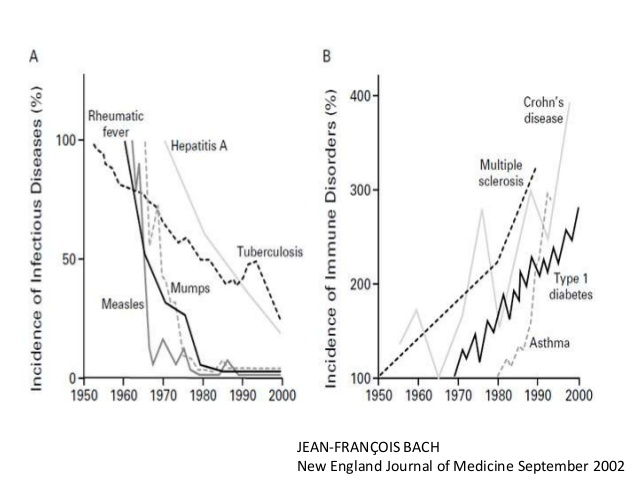
\includegraphics[scale=0.5]{img/allergie_infection.jpg}\hfill
\end{center}
\caption{Incidence des maladies infectieuses et auto-immunes en Europe au cours du temps. [@]}
\label{hyigienisme}
\end{figure}


Les récentes méthodes d'exploration de ce monde microscopique comme le séquençage haut débit ont permis aux bactéries de retrouver leurs lettres de noblesse.
Elles sont présentes partout et jouent le premier rôle dans le fonctionnement des écosystèmes. Elles sont par exemple impliquées dans le cycle de l'azote en permettant à la biomasse d'absorber le diazote atmosphérique. Les bactéries sont dans ce sens, la source primaire permettant aux organismes de construire leurs protéines et leurs ADN.
Elles peuvent vivre dans les milieux les plus inhospitaliers. Les archées (anciennement archéobactérie) peuvent résister à des conditions d'acidités et de températures exceptionnelles. On les retrouve dans les fonds océaniques privés de lumière où elles  sont la seule source d'énergie pour la faune en utilisant la chimiosynthèse à l'instar de la photosynthèse. les archées nous ont par ailleurs éclairés sur l’origine des eucaryotes. \footnote{Le génome des archées est composé d'introns comme chez les eucaryotes} et nous ont permise un bond de géant en biologie moléculaire \footnote{La Taq polymérase est une enzyme d'archée qui résiste à de hautes températures utilisées dans les PCR}.\\
L'homme ne fait pas exception. La majorité des bactéries ont longtemps été indétectables par les méthodes de culture classiques. Mais à présent, les régions anatomiques autrefois considérées stériles foisonnent de bactéries. 
Elles sont retrouvées dans tous les territoires du corps exposé ou elles forment des communautés.
La peau est colonisée par \textit{Propionibacterium}, \textit{Corynebacterium} et \textit{Staphylococcus} \citep{Beck}. Le vagin contient des \textit{Lactobacille} et la bouche principalement du \textit{Streptococcus}\cite{Beck}.
L'intestin est une flore bactérienne dominée par les anaérobies pouvant représenter jusqu'à 2 kg du poids corporel \citep{Beck}.
En échange de son hospitalité, le microbiote contribue au bon fonctionnement de son hôte. Il aide à la digestion en dégradant par exemple les sucres du lait maternel chez le nouveau-né[@bifidus]. Il participe à la synthèse de vitamine essentielle (K, B12,B8)[@ref]. Il éduque notre système immunitaire et fait barrière à tout nouvel agent pathogène.
Toute défaillance de notre microbiote ou \textit{dysbiose}, peut être délétère pour notre santé. La liste des affections associées est longue. On y retrouve la maladie de Crohn[@], la maladie coeliaque[@], le cancer de l’intestin[@], le syndrome du côlon irritable[@], l’obésité[@], le diabète de type 1[@], l’asthme[@], l’eczéma[@], la sclérose en plaque[@], la polyarthrite rhumatoïde[@], la maladie d’alzheimer[@] et même l’autisme[@]. \\
La colite à \textit{Clostridium Difficile} est un exemple de dysbiose avec une application clinique. La destruction de la flore intestinale par des antibiotiques donne l'opportunité à \textit{Clostridium Difficile} de s'installer. Un des traitements proposés est la transplantation fécale visant à régénérer le microbiote du patient. \\
Le microbiote amène donc à reconsidérer notre individualité. Nous ne sommes plus seulement un organisme multicellulaire composé d'un seul génome. Mais plutôt un écosystème où cellules eucaryotes et micro-organismes vivent en symbiose. Cette relation n'étant pas figée dans le temps et pouvant varier entre le commensalisme, le parasitisme et le mutualisme. Les dernières études estiment que pour chaque individu il y a environ 30 billions de cellules humaines pour 39 billions de cellules microbiennes[@]. En associant les gènes bactériens, le génome d’un humain passe de 23 000  à 3,3 millions[@] de gènes avec toute la complexité des interactions que cela engendre[@]. Les scientifiques ont attribué le nom d’\textit{holobionte} à cet écosystème vivant. L'ensemble des génomes est appelé \textit{hologénome}. \\
Il faut toutefois rester prudent quant au rôle donné aux microbiotes et éviter de tomber dans l'excès. Nombreuses sont les publications scientifiques qui se contredisent ou qui confondent corrélation et causalité. Ces publications ont même conduit à la création du hashtag humoristique sur Twitter: \textit{\#GutMicrobiomeAndRandomSomething}. 
Les études sur le microbiote nécessitent d'être étayé par des études fonctionnelles afin de trouver des relations de cause à effet. Les corrélations doivent être réalisées sur des populations plus grandes avec un suivi dans le temps plus important. Les nouvelles technologies de séquençage haut débit vont dans ce sens en collectant toujours plus de données.\\
Il est encore trop tôt pour dire si cette science va révolutionner la médecine de demain ou s’ il s'agit d'un effet de mode. Mais au regard de l'évolution biologique, il y a fort à parier dessus. Car, ne l'oublions pas, ce sont bien des anciennes bactéries, qui permettent à l'ensemble de nos cellules de respirer et que nous appelons maintenant des mitochondries (Figure \ref{mitochondrie}). 

\begin{figure}[ht]
\begin{center}
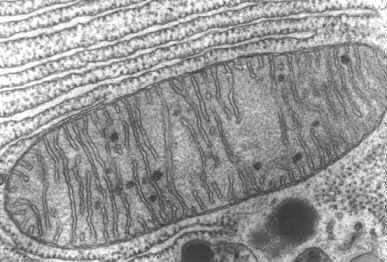
\includegraphics[scale=0.5]{img/mitochondrie.jpg}\hfill
\end{center}
\caption{La mitochondrie est l'exemple de symbiose ultime entre eucaryote et procaryote}
\label{mitochondrie}
\end{figure}



\newpage

\section{Définition}
\subsection{Termes utilisés en écologie}

\begin{description}
  \item[Le microbiote] est l’ensemble des micro-organismes (bactéries, levures, champignons, virus) vivant dans un environnement donné.
  
\item[Le microbiome] s’emploie selon deux définitions. En français, le microbiome est l'environnement qui héberge le microbiote. Dans sa définition anglo-Saxonne, le microbiome fait référence à l’ensemble des génomes microbiens contenus dans un environnement. 
De façon générale, le microbiome est associé aux génomes bactériens. Les termes de Virome et de Mycobiome sont utilisés pour les génomes viraux et mycosiques. 

\item[La biocénose] est le terme écologique dans un sens large désignant l'ensemble des organismes vivants dans un environnement appelé \textbf{Biotope}. Biocénose et biotope forment ensemble un \textbf{écosystème}.

\item[Une symbiose] est une association durable entre deux organismes. Leurs relations peuvent être mutualiste, parasitaire ou commensale.

\item[La métagénomique] est une méthode d’étude du contenu en ADN présent dans un milieu grâce aux techniques de séquençage haut débit. Contrairement à la génomique qui s’intéresse au génome d’un individu, la métagénomique s’intéresse aux génomes d’une population d’individu.
Dans son sens strict, la métagénomique correspond à l’étude de l’ensemble des séquences d'ADN. L’analyse d’un seul gène, comme celui de l’ARN 16s est associé à tort au terme métagénomique, mais son usage reste courant. On lui préférera le terme de \textbf{metagénétique}



\item[Un OTU] (\textit{Operational taxonomic Init}) est un terme utilisé en phylogénie, désignant un groupe d’individu proche faisant souvent référence à l’espèce dans la classification de Linée.
En microbiologie, un OTU est défini par un groupe d’individu ayant une similarité dans leurs séquences d'ARN 16s supérieur à 97\%.

\item[L'Abondance] absolu est le nombre de séquences d'ADN d'un OTU retrouvé dans un échantillon. 
L’abondance relative est le pourcentage en séquences d'ADN d'un OTU retrouvé dans un échantillon. Ce dernier permet de rendre les échantillons comparables entre eux.

\item[La table des OTU] correspond à un tableau à double entrée contenant l’abondance par OTU  et par échantillon. Dans le tableau suivant, l'échantillon 1 contient 68\% de l'OTU 1.

\begin{figure}
\begin{center}
\begin{tabular}{|l|c|c|c|c}
  \hline
   & échantillon 1 & échantillon 2 & échantillon 3  \\
  \hline
  OTU 1 & 68\% & 12\% & 25\% \\
  OTU 2 & 40\% & 24\% & 25\% \\
  OTU 3 & 28\% & 64\% & 50\% \\

  \hline
\end{tabular}
\end{center}
\caption{La table des OTUs}
\end{figure}

\item[La diversité alpha] est une mesure de biodiversité au sein d’un échantillon. Elle correspond à l’étude d’une colonne dans la table des OTUs. Plusieurs indicateurs de diversité alpha existent.

\item[La diversité bêta] est une analyse descriptive de la biodiversité entre plusieurs échantillons. Elle correspond à l’étude de l’ensemble de la table des OTUs. L’approche la plus courante est de réaliser une analyse multivariée par des méthodes d’ordination. Il s’agit de représenter un graphique à n dimensions, impossible à dessiner, en le projetant dans un espace à deux ou trois dimensions.

\item[La richesse] est le nombre d’espèces présent dans un échantillon. Les deux échantillons suivant ont une richesse de 2.

échantillon 1  : 4 Streptoccus , 4 Escherichia  \\ 
échantillon 2 : 432 Streptoccus, 12 Escherichia 

\item[L'uniformité / équitabilité] indique si les espèces d’un échantillon sont réparties uniformément.
L'uniformité du premier échantillon est plus grande que la seconde

échantillon 1  : 50 Streptococus , 50 Escherichia  \\ 
échantillon 2 : 432 Streptoccus, 12 Escherichia 


\item[L'indice Chao1] est une estimation de la richesse réelle (in vivo) par rapport à la richesse observée (in vitro). Cet indice part du principe que si l’échantillon contient beaucoup de singletons ( OTU détecté une seule fois), il est fort probable que la richesse réelle soit plus grande que la richesse de l’échantillon. La formule est la suivante.
\begin{equation}
A = B
\end{equation}

\item[L'indice de Shannon] est un indicateur évaluant à la fois la richesse et l’uniformité dans un échantillon. Il se calcule de la même façon que l’entropie de Shannon.

\begin{equation}
A = B
\end{equation}

\item[L'indice de Simpson] est un indicateur évaluant la probabilité que deux individus sélectionnés aléatoirement dans un échantillon donné soient de la même espèce. La formule est la suivante.

\begin{equation}
A = B
\end{equation}


\item[La courbe de raréfaction] est utilisé pour déterminer si la profondeur de séquençage est suffisante pour caractériser la diversité d’un échantillon.
Pour générer cette courbe, des groupes de reads de taille croissante (1…n) sont tirés aléatoirement sans remise. Le groupe est reporté sur l'axe X et le nombre d’OTU correspondant est reporté sur l’axe Y.
Une courbe s’aplatissant indique une bonne profondeur de séquençage \citep{Dickson2014} AMD \citep{Beck}

\end{description}


\subsection{Termes utilisés en bioinformatique}

\begin{description}
\item[Pipeline] 
Un pipeline est un ensemble d'étapes de calcul informatique. Chaque étape prend en entrée des fichiers pour en produire des nouveaux dans sa sortie. On peut comparer cela aux étapes d'une recette de cuisine. Sans parallélisation, un cuisinier (le processeur) doit attendre de faire fondre le beurre avant de battre les œufs en neige ( Exécution synchrone). En parallélisant, le cuisinier peut réaliser plusieurs étapes en même temps. Battre les œufs pendant que le beurre fonde.( Exécution asynchrone). 
Maintenant si l'objectif est de produire 188 gâteaux (188 analyses) et que l'on dispose de 64 cuisiniers ( 64 processeurs), l'organisation des tâches devient complexe si l'on veut maximiser le rendement. Pour cela, on dispose d'outils comme snakemake, qui permettent de générer un graphe des étapes( direct Acyclique Graph) et de trouver la meilleure façon d'optimiser les taches entre les différents cuisiniers (processeur). 

\item{NGS} ... 

\item[Un read] est un terme bio-informatique désignant une séquence d’ADN issue d’un séquençage haut débit. Selon les technologies, les reads varient entre 150 et 300 paires de bases.

\item[librarie] ... 

\item[Un fichier fastq] .....

\item[Un fichier fasta] .....

\item[Un fichier biom] .....

\item[R] .....


\end{description}

\newpage

\setcounter{page}{1}

\section{Introduction}
\subsection{La mucoviscidose}
\subsubsection{Une maladie génétique}
La mucoviscidose est une maladie génétique autosomique récessive grave qui frappe en France 1 naissance sur 5400 [@]. La Bretagne est la région la plus touchée avec une prévalence de 1/3000[@].
La loi de Hardy Weinberg estime qu’en Bretagne 1 patient sur 25 est porteur de la mutation à l’état hétérozygotes[@Heterozygote davantage]. Cette haute prévalence s’explique probablement par un effet fondateur associé à un avantage sélectif pour les individus porteurs de l’allèle muté. \footnote{Plusieurs hypothèses ont été proposées, notamment lors des grandes épidémies de choléra en diminuant les pertes hydriques. D’autres suggèrent qu'il s'agit d'une pléiotropie antagoniste.[@]} \\
Le gène CFTR impacté se situe sur le chromosome 7 en position q31.2. Il est constitué de 27 exons pour 250 188 [@] paires de bases. Il code pour un canal chlore AMP dépendant permettant les échanges des ions chlorures au niveau des membranes cellulaires[@]. Il est également impliqué dans le transport du thiocynate (SCN-) et des bicarbonates (HCO3-)[@]. \\
On dénombre à ce jour 2017 mutations mises en cause dans la mucovicidoses[@]. La perte d’une phénylalanine en position 508 par délétion du triplet c.1521-1523delCTT (anciennement $\Delta$F508) cause à elle seule 80\% des mucoviscidoses.
Ces mutations sont responsables d’une protéine défectueuse ou d’une absence de canaux sur les membranes cellulaires. \\
Cliniquement, la mutation entraîne une insuffisance pancréatique exocrine et une infertilité par disparition des canaux déférents. Des signes digestifs, hépatiques et articulaires sont également retrouvés.
L'atteinte de la fonction respiratoire est la plus bruyante. En effet au niveau de l’épithélium broncho-pulmonaire, l’absence d’un CFTR fonctionnel est à l’origine d’une déshydratation du mucus le rendant plus visqueux et empêche les cils bronchiques de jouer leurs rôles.[@]\\
La forte prévalence de la maladie nécessite de réaliser un dépistage précoce chez tous les nouveaux nés (test de Gutri) afin d’adapter au plus tôt la prise en charge. Seul le test à la sueur permet de poser le diagnostic. Le dépistage prénatal basé sur l’ADN circulant est actuellement à l’étude[@]. Le traitement repose avant tout sur une prise en charge respiratoire (kinésithérapie, dorasse, antibiothérapie).
Les recherches en thérapies génétiques sont encourageante[HAS].
L’Ivacaftor est le seul traitement à ce jour qui agit directement sur le CFTR. Mais concerne uniquement certaine mutation rare comme la G551D.[has]La greffe pulmonaire est le dernier recours.

\subsubsection{Une maladie infectieuse}

L’atteinte pulmonaire dans la mucoviscidose est caractérisée par des réactions inflammatoires qui dégrade progressivement la fonction respiratoire. Plusieurs pathogènes sont impliqués. Chez les jeunes enfants, \textit{Haemophilus influenza} et \textit{Staphilococcus Aureus} sont le plus souvent responsable. \textit{Burkolderia Cepace} et \textit{Stenotrophomonas Maltophilia} sont retrouvés parmi les sujets plus âgé.
Mais c’est \textit{Pseudomonas Aeruginosa} qui caractérise l’atteinte pulmonaire dans la mucoviscidose en marquant un tournant décisif dans l’évolution de la maladie. Ce bacille aérobie stricte est un germe de l'environnement rarement retrouvé parmi les patients sains[@]. En revanche, dans la mucoviscidose, il est mis en évidence chez 60\%[@] des patients jeunes, et plus de 90\% des patients adultes[@].\\
La primocolonisation à \textit{Pseudomnas Aeruginosa} est difficilement détectable, mais semble avoir lieu tôt dans l’enfance[@]. Il y a ensuite une phase de latence, variable entre les individus, marquée par des épisodes d’exacerbations et de rémissions. À ce moment, l’éradication[@] par des antibiotiques reste possible.
Puis survient le passage à la chronicité. \textit{Pseudomnas Aeruginosa} s'adapte à son milieu et s’installe à long terme. Il perd certains caractères de virulence, mais devient résistant aux antibiotiques[@]. Son phénotype change. Il se transforme pour devenir mucoïde en sécrétant un film d’alginate qui le protège du système immunitaire. Les mécanismes sous-jacents à cette adaptation sont ingénieux. La forte densité en bactérie est responsable d’activation de certains gènes par un processus appelé \textit{quorum sensing}[@]. Un processus dans lequel chaque bactérie communique avec ses voisines par des signaux.
Le génome de \textit{Pseudomnas Aeruginosa} devient aussi hyperpermutable afin de présenter une plus grande diversité génétique au regard de la sélection naturelle\footnote{En biologie évolutive, il s'agit d'évolvabilité}. \\
À ce stade, le traitement antibiotique n’est plus curatif et l'évolution tend inexorablement vers un déclin de la fonction respiratoire. \\
L'approche clinique est donc préventive afin de retarder le passage à la chronicité. Elle vise à éliminer \textit{Pseudomnas Aeruginosa} dès qu'il est détecté en culture. Une surveillance rapprochée des patients avec un prélèvement mensuel ou bimensuel est préconisée selon l'HAS[@]. La culture étant peu sensible, d’autres méthodes d'identification peuvent être employées. La détection des anticorps anti-pyocyaniques par ELISA a montré peu de sensibilité [@].
La PCR ciblée associant les protéines bactériennes \textit{OPRL1} , \textit{GYRB1} et \textit{ECFX1}  s’est montrée plus sensible et plus spécifique que la culture[@]. \\
En pratique, la colonisation chronique est définie lorsque 3 expectorations sont rendues positives en culture, successivement au cours d’un suivi mensuel ou bimensuel[@].
Une autre classification, celle de Lee a montré une forte liaison clinico-biologique. Elle est composée de 4 groupes :  
\begin{description}
\item[groupe chronique] > 50\% des cultures sont positives sur 12 mois
\item[groupe intermédiaire] $\leq$ 50\% des cultures sont positives sur  12 mois
\item[groupe Free] Toute culture négative sur 12 mois, avec des antécédents
\item[groupe Nevers] Toute culture négative sur 12 mois sans antécédents 
\end{description}

On ne sait pas aujourd’hui pourquoi \textit{Pseudomnas Aeruginosa} s’installe préférentiellement chez les patients atteints de mucoviscidose. Plusieurs hypothèses ont été proposées : 

%----------------- REFORMULER -----------------
\begin{itemize}
\item La dysfonction ciliaire empêche les pseudo d’être viré par le haut
\item L’hypersalinité du film muqueux désactive les peptides antimicrobiens
\item Le CFTR est un récepteur de pyo qui les internalise et les viré
\item L’inflammation de  l’epithelimum augmente les métabolites qui permettent de se développer.
\item Alanine et l’acta sont une source de carbone pour le pyo.
\item Le microbiote influence la colonisation
\item Le pyo stimule le Systeme immunitaire pour virer tous les autres concurrents 
\end{itemize}




\begin{figure}[ht]
\begin{center}
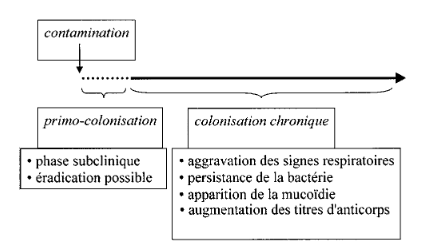
\includegraphics[scale=0.8]{img/chronic.png}\hfill
\end{center}
\caption{Infection pulmonaire à pyo dans la mucoviscidose. ref []}
\label{bach}
\end{figure}


\subsection{Le microbiote pulmonaire}

Bien qu'il soit en contacte avec le milieu extérieur, l’arbre respiratoire (comprenant la trachée, les bronches et les alvéoles) a longtemps été considéré comme stérile avec les méthodes de culture classique. Il a fallu attendre l’avènement du séquençage haut débit pour mettre en évidence le microbiote pulmonaire[ref Host-microorganism 1-3].
Le microbiote pulmonaire est beaucoup moins abondant que le microbiote digestif. Il est constitué d’une flore dynamique provenant de l’air ambiant, des voies supérieures,  mais aussi du tube digestif par des micro-aspirations.[@]
Le microbiote pulmonaire est dominé par le phylum des \textit{Firmicutes} (\textit{Streotpococcus}) et des \textit{Bacteroidetes} (\textit{Prevotella}). Les genres retrouvés majoritairement sont \textit{Streptococcus}, \textit{Prevotella}, \textit{Fusobacteria}, \textit{Veillonella}, \textit{Haemophilus}, \textit{Neisseria} et \textit{Porphyromonas}.
L’arbre respiratoire étant en continuité direct avec les voies aériennes supérieur, certains genres bactériens sont communs, comme \textit{Streptococcus}, \textit{Staphylococcus}, \textit{Haemophilus} et \textit{Moraxella}. Tandis que d’autres genres comme \textit{Corynébactérium} et \textit{Dolosigranulum} ne sont retrouvés qu’au niveau du nez et de l'oropharynx. \\
Le microbiote pulmonaire varie dans l’espace et le temps. \\
Dans l’espace, du fait de sa structure, certaines régions de l'arbre bronchique peuvent présenter des microbiotes différents. Un prélèvement au niveau d'un foyer infectieux se distinguera nécessairement d'un foyer sain. Il existe également des différences physico-chimiques selon la région pouvant sélectionner des espèces. Les cavernes tuberculeuses par exemple se trouvent essentiellement dans le lobe supérieur en raison d'une concentration en oxygène plus élevé qui favorise ce bacille aérobie stricte. \\
Le microbiome varie dans le temps... 
Declin de la diversité alpha avec l'age .... probablement a cause des exacerbations multiple et du traitement
Le microbiote est variable entre les individus ... \\
Le microbiote est corrélé à la pathologie respiratoire. Plusieurs études suggèrent une différence entre patients sains et patients asthmatiques, BPCO ou atteint de mucoviscidose ...... [@].
Chez les muco, augmentation de la richesse et diminution de la diversité 
Chez les muco, augmentation des germes opportuniste par rapport au commensaux ( data mining paper)


\subsection{Exploration du microbiote pulmonaire}
%(http://bacterioweb.univ-fcomte.fr/bibliotheque/remic/08-Bronc.pdf) ==> A LIRE COOURS BACTERIO

\subsubsection{Méthode de prélèvement}
Le microbiote respiratoire est exploré en séquençant l'ensemble des ADN présent dans un échantillon. 
Toutes les méthodes de recueils sont possibles, mais les prélèvements protégés (combicath, LBA) sont recommandés afin
d’éviter une contamination par les voies supérieures. Dans le cas contraire (ECBC) on peut évaluer la qualité du prélèvement en comptant le nombre de cellules épithélium ( normalement bas ) et de polynucléaire ( normalement haut ) dans le poumon. La meilleure méthode de prélèvement étant le prélèvement in situ réalisable lors des greffes pulmonaires.

\subsubsection{Séquençage haut débit}
% Baisse du coup du sequencage ... %
Grâce à son haut débit, Le séquençage de nouvelle génération permet de séquencer l'ensemble des ADN présent dans un échantillon respiratoire et ainsi déterminer sa composition en bactérie. À titre d'exemple, un séquenceur Sanger classique permet de lire des fragments d'ADN d'environ 800 pb parallélisable jusqu'à 96 fois en augmentant le nombre de capillaire sur la machine. 
À l'inverse, un séquenceur de nouvelle génération lit des fragments plus courts de l'ordre de 150pb. Mais cette lecture peut être parallélisé jusqu'à 20 billions de fois en un seul run sur un illumina Novaseq. \\
2 stratégies de séquençages sont utilisées en écologie microbienne:  \\
\textbf{La stratégie shogun} consiste à séquencer l'ensemble des  ADN présents dans l'échantillon sans discernement, que ce soit humain ou bactérien. Les séquences sont filtrées puis les génomes bactériens sont reconstruits par des méthodes bio-informatiques complexes. \\
\textbf{La stratégie Amplicon} est moins coûteuse sur le plan de l'analyse. Il s'agit d'amplifier un gène uniquement bactérien et suffisamment variable pour discriminer une espèce. Pour les bactéries, il s'agit de l'ARN 16S.\\
L'ARN 16S est un ARN non codant participant à la structure de la petite sous unité des ribosomes bactériens. Il est composé de 1500 nucléotides et forme plusieurs boucles dans sa structure secondaire (Figure \ref{ARN16S}). 
L'alignement des séquences d'ARN 16S entre plusieurs espèces met en évidence des régions constantes et 9 régions variables (Figure \ref{ARN16SVariation}). Les régions constante permette de concevoir des amorces s'hybridant sur tous les ADNs bactériens. Les régions variables apportent la spécificité taxonomique permettant d'identifier l'espèce bactérienne.
% Les études de [@] ont montrée que certaine région variable apportent plus de spécificité.

\begin{figure}[ht]
\begin{center}
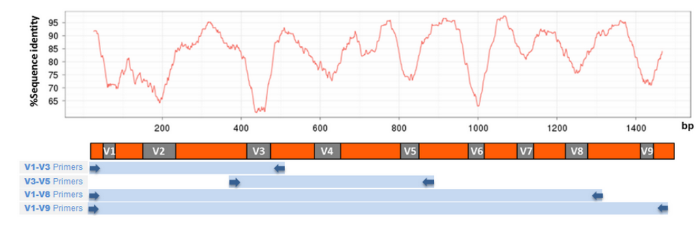
\includegraphics[scale=0.8]{img/ARN16S_variation.png}\hfill
\end{center}
\caption{région constante et variable de l'ARN 16S}
\label{ARN16SVariation}
\end{figure}

\begin{figure}[ht]
\begin{center}
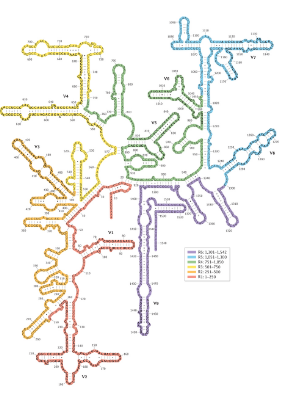
\includegraphics[scale=0.8]{img/ARN_16S.png}\hfill
\end{center}
\caption{Structure secondaire de l'ARN 16S}
\label{ARN16S}
\end{figure}


En séquencant l'ensemble des génomes bactériens, la stratégie \textit{shotgun} est plus informative car elle permet de prédire la fonction d'un microbiote. En effet, les transferts génétiques horizontaux amènent à dissocier l'espèce de sa fonction. 2 bactéries d'une même espèce peuvent avoir des fonctions différentes. L'inférence fonctionnelle à partir de la deuxième stratégie est possible mais déconseillé[@].  
La stratégie 16S reste toutefois une méthode simple pour décrire les populations bactériennes présentes. C'est cette stratégie qui a été utilisée dans notre étude. 



\subsection{Objectif de l'étude Mucobiome}
L'objectif de notre étude est de savoir si le microbiote respiratoire influence la primo colonisation à \textit{Pseudomnas Aeruginosa}. 
Pour cela, nous avons suivi pendant 3 ans,  une cohorte de 47 patients atteints de mucoviscidoses sans infection chronique. 
L'exploration de leurs microbiotes par la stratégie 16S a été réalisée à partir d'expectorations bronchiques obtenues dans le cadre de leurs suivis. 
À partir des données générées par le séquençage, nous avons effectué l'étude descriptive et analytique de leurs microbiotes en créant un pipeline bio-informatique dédié. 

\section{Matériel et Méthodes}
\subsection{Recueil des données}

47 patients atteints de mucoviscidose ont été suivis sur 3 ans (2008-2011) dans une étude prospective multicentrique (Nantes,Brest,Roscoff) appelée mucobiome.
La CPP VI-Ouest et le comité d’éthique du CHRU de Brest ont approuvé le protocole. Tous les patients ( ou les parents pour les mineurs) ont signé un consentement éclairé. Le protocole a fait l’objet d’une déclaration de biocollection à l’ARS et au MESR (n DC-2008-214).\\
Les ECBC des patients ont été recueillies lors des séances de kinésithérapie respiratoire tous les 3 mois, suivant le calendrier des recommandations officielles. En pratique, sur l’ensemble de la cohorte suivie, l’intervalle médian entre 2 consultations a été de 3,4 mois.
Les patients devaient avoir un génotype CFTR et un test à la sueur positif. Les transplantés ont été exclus de l’étude.
Une culture positive à \textit{Pseudomnas Aeruginosa} était un critère de non-inclusion. Si pendant l’étude, une culture revenait positive à \textit{Pseudomonas Aeruginosa}, le patient était sorti de l’étude pour être réinclus 1 an après en l’absence de colonisation chronique. 15 patients ont été ainsi réinclus.
Chaque patient a été répertorié dans la catégorie Free ou Never (Lee et ale 2003). D’autres données ont également été recueillies ( Figure \ref{summary} ).
Au total , 188 échantillons ont été récoltés, soit en moyenne 4 échantillons par patients.
Pour chaque échantillon, une culture a été réalisée en suivant les procédures standards [@]. Une qPCR ciblant \textit{Pseudomnas Aeruginosa} a parallèlement été réalisée en combinant les marqueurs gyrB/ecfX conçus au laboratoire[@].


\begin{figure}[ht]
\begin{center}
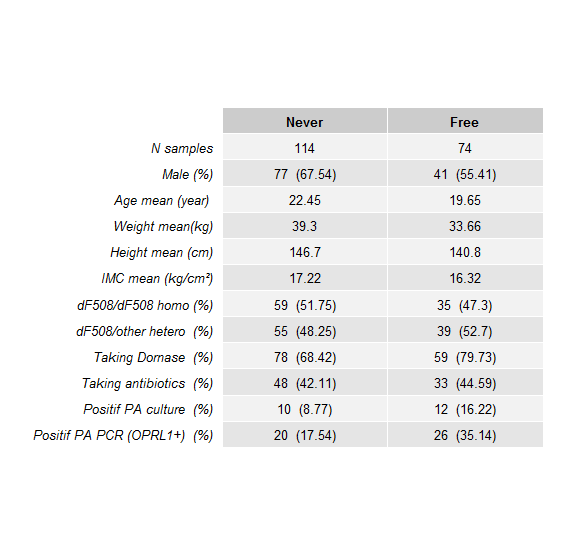
\includegraphics[scale=0.8]{img/summary.png}\hfill
\end{center}
\caption{Données associés par échantillons ( à refaire par patients)}
\label{summary}
\end{figure}



\subsection{Extraction de l’ADN}

Les échantillons ont été liquéfiés avec du Dithiotrétiol. Les protéines ont été dégradées avec une Protéine kinase.
Les parois bactériennes ont été fragmentées par sonication. (DTT par sonication (Elamsonic S10, Singen, Germany). Après 10 min de centrifugation, L’ADN a été extrait à partir du culot via QUIAamp DNA Minikit ( Quagen).
Les extraits d’ADN ont été envoyés pour séquençage par un prestataire GATC.

\subsection{Séquençage}
La librairie \footnote{l'ensemble des fragments d'ADN à séquencer} a été généré en amplifiant la région V3-V5 à l’aide du couple d’amorces  \textit{forward(CCTACGGGAGGCAGCAG)} et \textit{reverse(CCGTCAATTCMTTTRAGT)} et du kit MiSeq Reagent Kits v3. \\
Le séquençage a été réalisé sur Illumina MiSeq. Un couple de séquence chevauchant de 300pb est produit (Figure \ref{illumina}). Après fusion du couple, le séquençage permet de lire les 535 pb correspondant à la région V3-V5.\\
Environ 25 millions de reads sont produits par run MiSeq. En multiplexant à l’aide de 94 index, les 188 échantillons ont été séquencé sur 2 runs pour produire 188 x 2 fichiers fastq.

\begin{figure}[ht]
\begin{center}
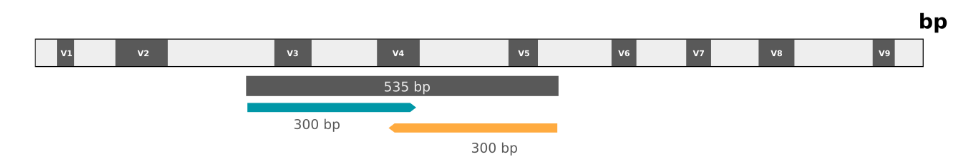
\includegraphics[scale=0.6]{img/illumina.png}\hfill
\end{center}
\caption{le couple de séquence de 300pb permet de recouvrir l'ensemble de la région V3-V5}
\label{illumina}
\end{figure}


\subsection{Analyse bio-informatique}

L’analyse des 188 pairs de fichiers fastq a été réalisé grâce à un pipeline bio-informatique, appelé \textit{mucobiome}, conçu et tester dans le cadre de cette étude. Par rapport aux autres logiciels comme \textbf{QIIME} ou \textbf{MOTHUR}, le pipeline mucobiome est spécialisé dans l’analyse des données 16S. Il est également plus rapide en raison d’un très haut niveau de parallélisation permis grâce à  \textbf{Snakemake}. Cet outil modélise l'ensemble du pipeline sous forme d'un graphe direct acyclique (DAG) et le résout afin d'optimiser la parallélisation. \\
Le pipeline mucobiome prend en entrée, les 188 couples de fichiers fastq provenant du séquençage et produit un fichier BIOM contenant la table des OTUs. Les figures \ref{pipeline_trio} et \ref{dag} illustrent toutes les étapes du pipeline et sont décrites ci-dessous.



\begin{figure}[!ht]
\begin{center}
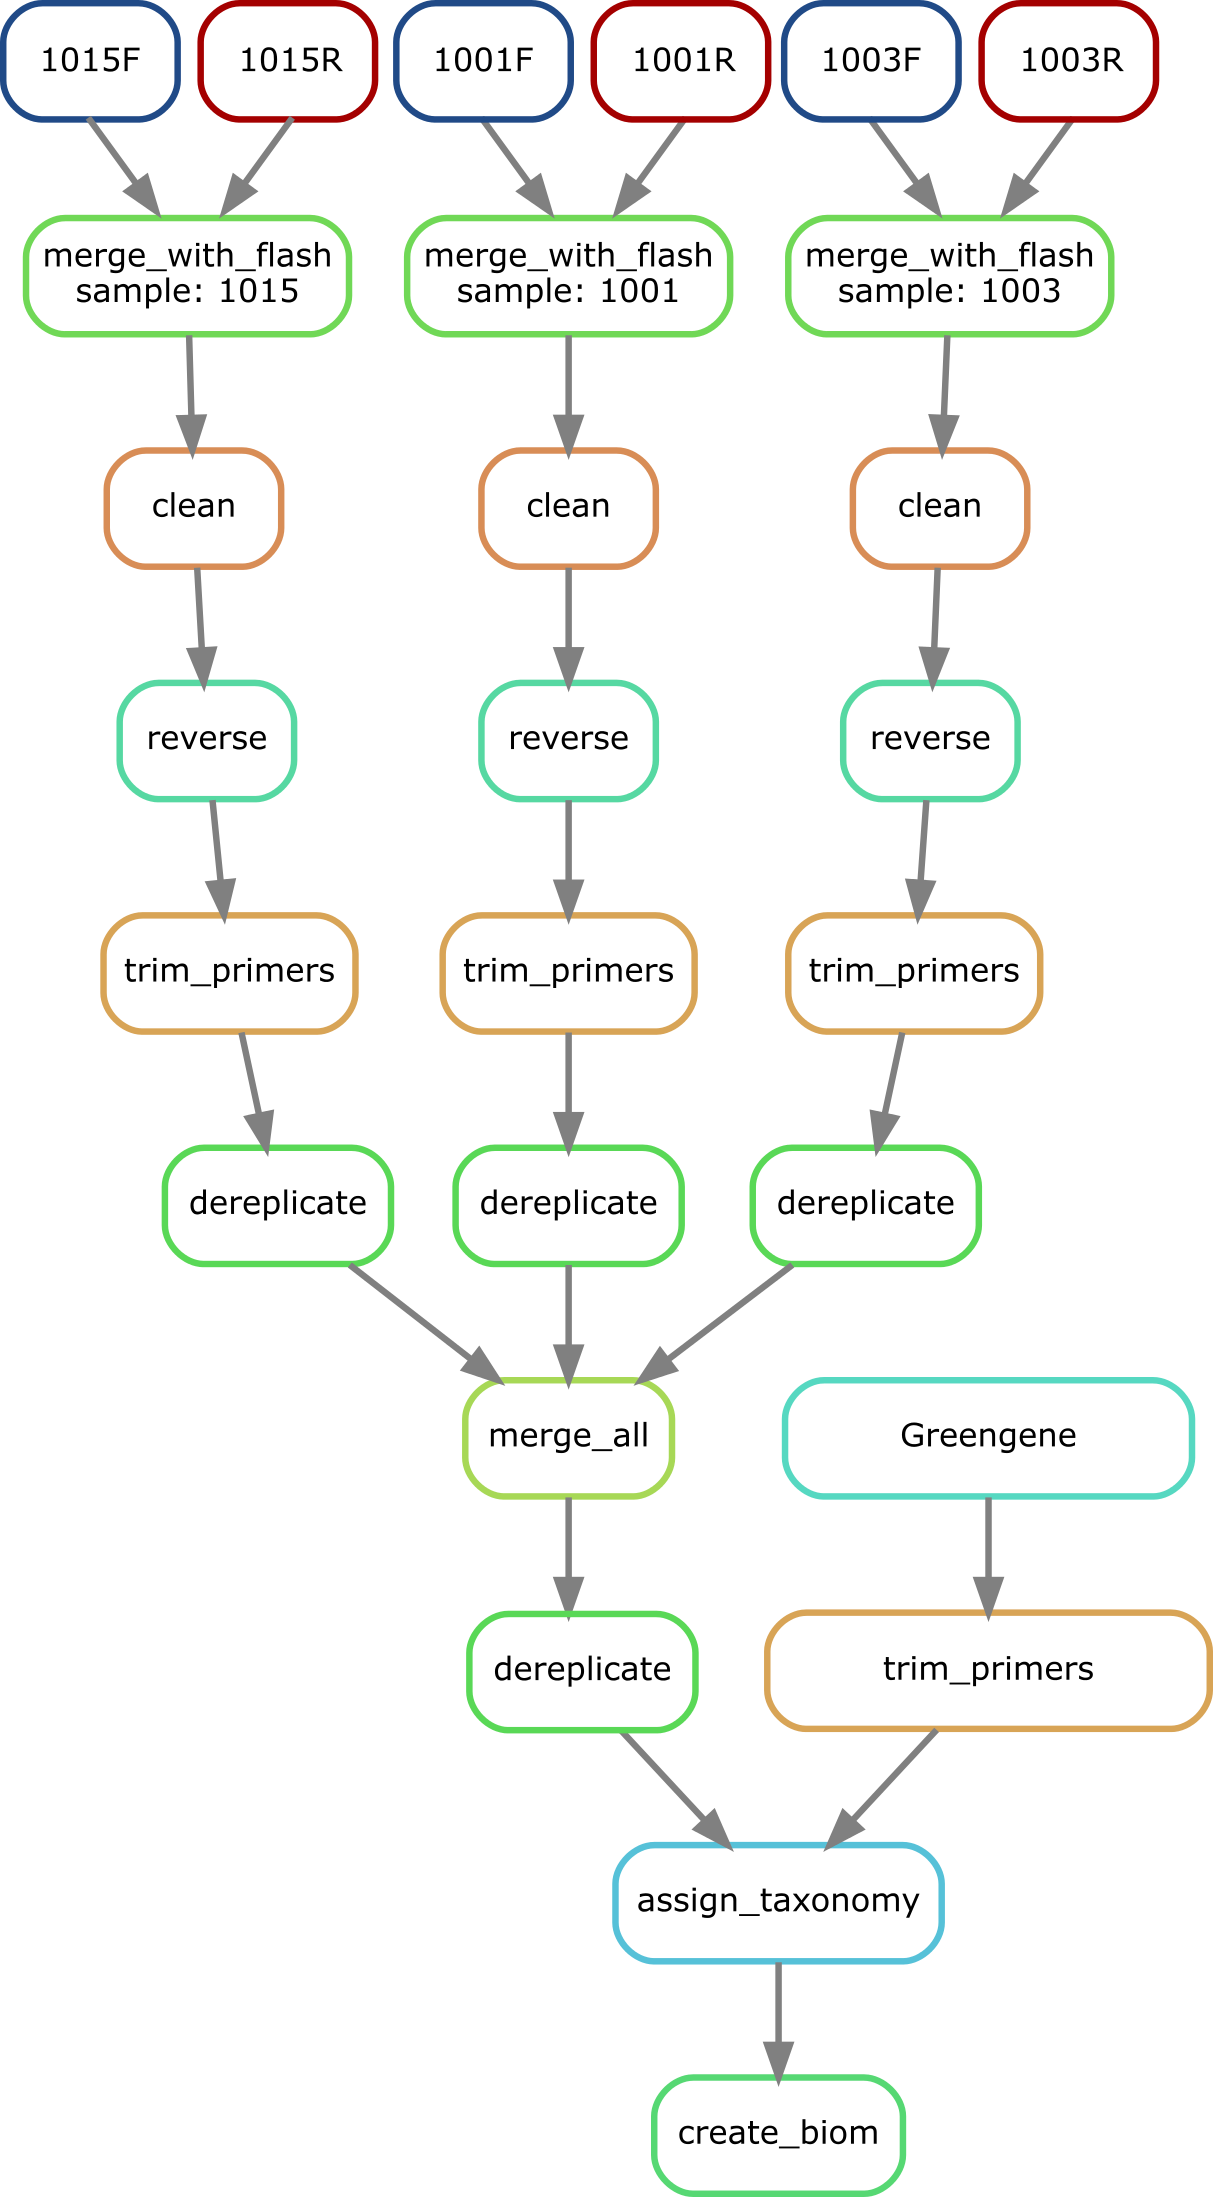
\includegraphics[scale=0.5]{img/pipeline_trio.png}\hfill
\end{center}
\caption{Graphe du pipeline simplifié sur 3 échantillons 1015, 1001 et 1003.\\ \textbf{merging}: Les reads pairs de 300 pb sont fusionnés  pour produire un fichier fastq contenant des reads de 535pb. \textbf{cleanning}: les reads de mauvaise qualité sont supprimés. \textbf{reversing}: les reads sont transformés en leurs séquences complémentaires pour pouvoir être alignés. \textbf{Trimming}: seule la séquence entre les primers V3-V5 est conservée. \textbf{dereplicating}: les séquences dupliquées sont retirées. \textbf{merging}: L'ensemble des séquences est regroupé dans un seul fichier. \textbf{Taxonomy assignent}: Les séquences sont alignées sur la base de données greengene. \textbf{create\_biom}: la table des OTU est créée }
\label{pipeline_trio}
\end{figure}


\begin{figure}[ht]
\begin{center}
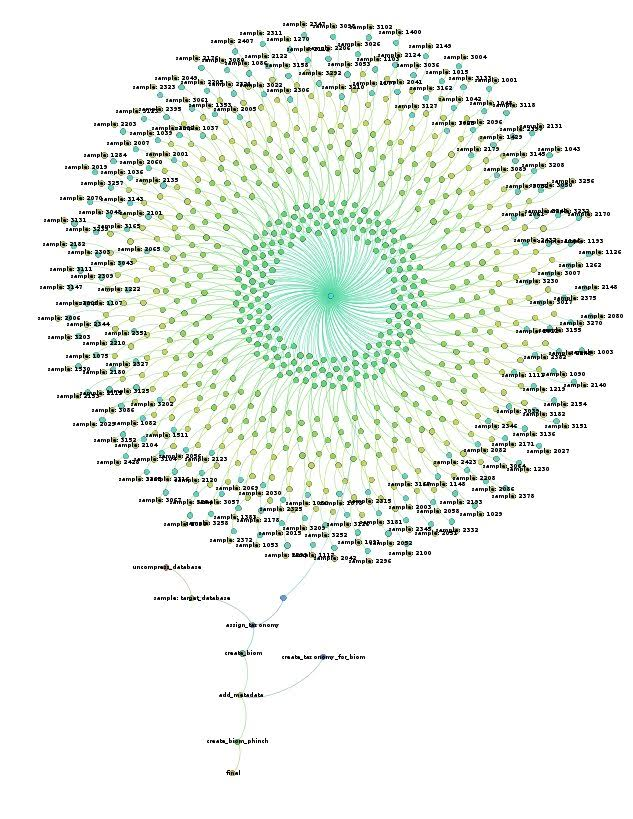
\includegraphics[scale=0.4]{img/dag.jpg}\hfill
\end{center}
\caption{le graphe du pipeline sur l'ensemble des échantillons}
\label{dag}
\end{figure}

% +++ RELECTURE 
\subsection{Étape du pipeline}
\subsubsection{Merging: Fusions des reads}\begin{center}\emph{ 2 fastq en entrée 1 fastq en sortie. } \end{center}

La première étape du pipeline consiste à fusionner le couple de fichier fastq afin de produire un seul fichier contenant des plus longues séquences de 535pb correspondant à la région V3-V5 de l’ARN 16S.
Le programme \textbf{Flash}[@] a été utilisé avec les paramètres par défaut. À partir de deux fichiers fastq, ce dernier recherche le meilleur alignement entre deux reads et produit 1 fichier fastq contenant les reads fusionnés.
Une analyse qualitative des reads a été réalisée avec FastQt\citep{Beck} avant et après fusions.

\subsubsection{Cleaning: Filtrage des qualités}\begin{center}\emph{1 fastq en entrée 1 fastq en sortie. } \end{center}

Les données de séquençage haut débit peuvent contenir beaucoup d'erreurs. Il est important de supprimer les reads de mauvaise qualité pour gagner en spécificité. ( expliquer la qualité).
Le filtrage des reads de mauvaise qualité est réalisé avec le programme \textbf{sickle}. Son algorithme repose sur l'utilisation d'une fenêtre glissante de taille définie ( par défaut : 20 Pb). Cette fenêtre glisse le long de la séquence et pour chaque position calcule la moyenne des scores de qualité dans cette fenêtre. Si successivement le score moyen passe sous un certain seuil, le read est supprimé. Les paramètres utilisés sont ceux par défaut. Un score de 20 avec une fenêtre glissante de 20pb. 
Une analyse qualitative des reads a été réalisée avec FastQt\citep{Beck} après le filtrage. 


\subsubsection{Reversing: Séquence complémentaire}\begin{center}\emph{1 fastq en entrée 1 fasta en sortie. } \end{center}

Les reads produits par le séquenceur ne sont pas orientés dans le même sens que la base de données \textit{greengene}. Pour permettre l'alignement, les séquences ont été remplacées par leurs séquences complémentaires grâce au programme \textbf{seqtk}. 
Par la même occasion les scores de qualités devenus inutiles sont supprimés. Les séquences sont sauvegardées dans un fichier fasta. 

\subsubsection{Trimming: Suppression des primers} \begin{center}\emph{1 fasta en entrée 1 fasta en sortie. } \end{center}

Pour permettre un alignement parfait entre les reads et la base de données, les primers sont retirés et seule la séquence V3-V5 est conservée. Cette étape est réalisée aussi bien pour les données du séquençage que  la base de données greengene.  
Le programme \textbf{cutadapts} est utilisé avec une tolérance de 0.1 par défaut. 

\subsubsection{dereplicating: Suppression des doublons}\begin{center}\emph{1 fasta en entrée 1 fasta en sortie. } \end{center}

Cette étape consiste à supprimer toutes les séquences doublons. En procédant ainsi, on s'assure de ne pas répéter l'assignement taxonomique plusieurs fois sur des reads identiques. Le nombre de reads dupliqué est conservé pour être pris en considération lors du calcul des abondances. Il s'agit d'une étape d'optimisation permettant d'économiser en temps de calcul. La déréplication a été réalisé avec \textbf{vsearch} et sa fonction \textit{--derep\_fulllength }

\begin{figure}[ht]
\begin{center}
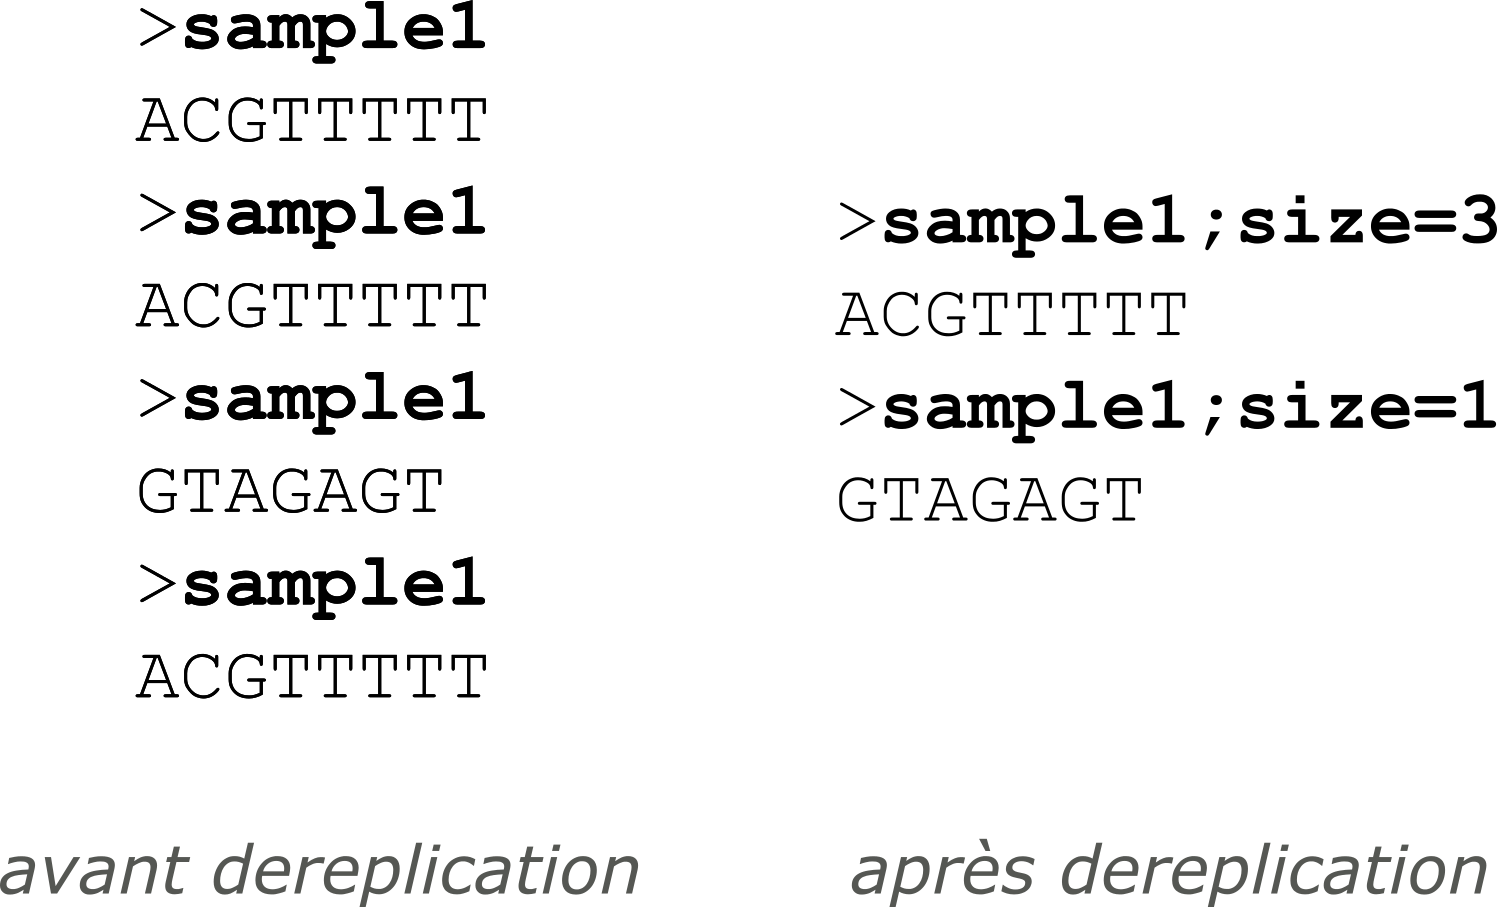
\includegraphics[scale=0.4]{img/dereplication.png}\hfill
\end{center}
\caption{Exemple de déréplication d'un fichier fasta}
\label{dereplication}
\end{figure}

\subsubsection{Assignement taxonomique} \begin{center}\emph{2 fasta en entrée,  1 fichier biom  en sortie. }\end{center} 

L’assignement taxonomique consiste à labelliser chaque read à son taxon. Nous avons utilisé la stratégie \textit{close référence} dont le rôle est de comparer chaque read à une base de données avec un seuil de 98\% de similarité. Cet algorithme est de complexité N. C'est-à-dire que le temps de calcul est directement proportionnel au nombre de reads testé. La base de données \textit{Greengene} version mai 2013  a été utilisé. Il s'agit d'un fichier fasta contenant 1 262 986 séquences et 203 452 OTUs. \\
L'autre stratégie d'assignement \textit{de novo} n'a pas été utilisée. Cette dernière, de complexité $N^{2}$, consiste à comparer les reads entre eux pour former des groupes. Elle s'emploie de préférence pour détecter les bactéries absentes des bases de données. \\
L'assignement taxonomique a été réalisé avec vsearch et sa fonction \textit{--usearch\_global}. 

\subsubsection{Analyse descriptive}
L'analyse de la table des OTUs a été réalisée avec R et le package phyloseq. 
Les OTUs ont été regroupé agrégé par genre.
la diversité globale et individuelle a été évalué à l'aide de plusieurs graphiques. L'ensemble des résultats est disponible à cette adresse : http://...  



\section{Résultat}
\subsection{Séquençage et pipeline}
\subsubsection{Données de séquençage}
Après démultiplexage, 188 x 2 fichiers Fastq ont été générés soit 2 fichiers pairs par échantillons.
La longueur des reads pour chaque fichier est de 301 paires de bases.
Au total, 115 002 297 reads ont été produits sur 2 runs MiSeq (Figure \ref{readcount}). Avec en moyenne 616 900 reads par échantillon. Un minimum de 61 422 reads pour l’échantillon 2154 et un maximum de 1 071 188 pour l’échantillon 3165. 


\begin{figure}[ht]
\begin{center}
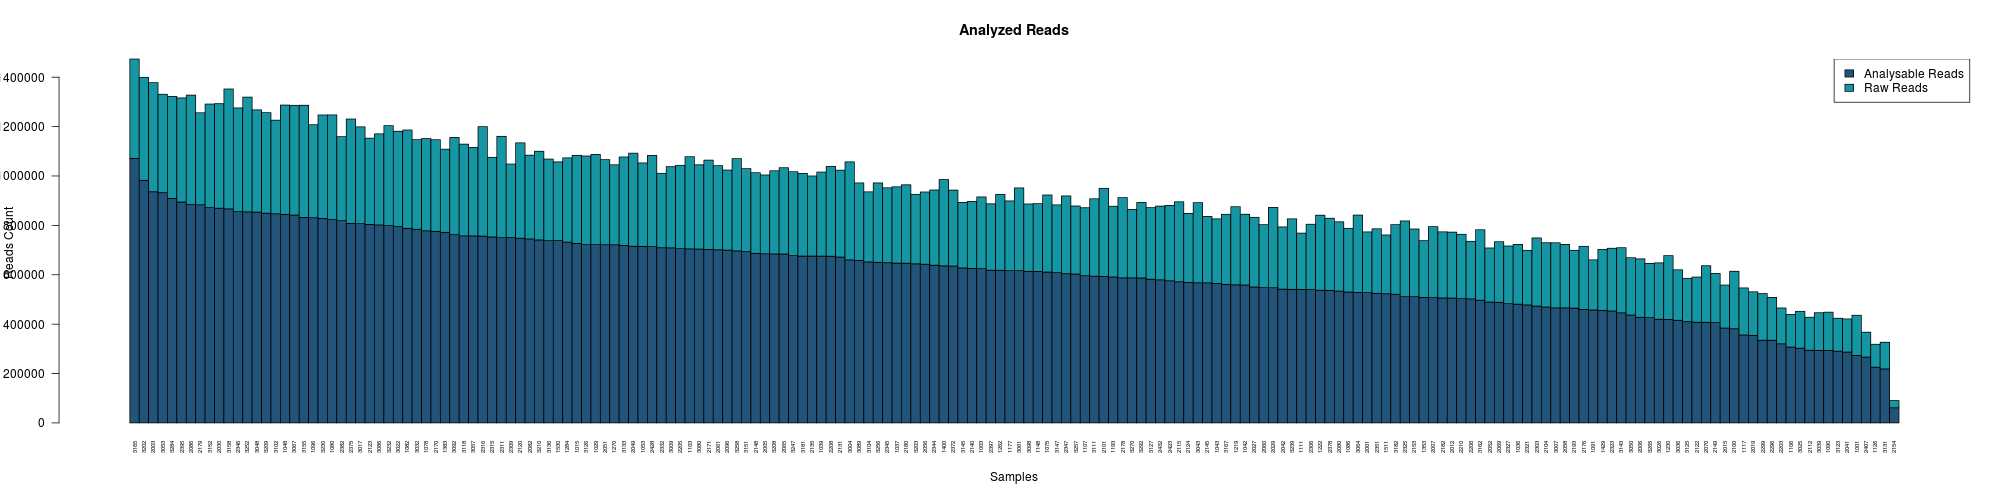
\includegraphics[scale=0.25]{img/pipeline.png}\hfill
\end{center}
\caption{Nombre de reads par échantillons}
\label{readcount}
\end{figure}


\subsubsection{Qualité des reads}
La figure \ref{fastqt} montre le profil de qualité des reads d’un échantillon avant fusion. Une baisse du score de qualité importante est observée à hauteur du 250ème nucléotide. Les 188 échantillons présentaient le même profil.
La figure \ref{fastqt_after} représente les scores de qualités d’un échantillon après fusions et après filtrage des reads de mauvaise qualité. Le chevauchement des reads pairs n'étant pas suffisant, une baisse de qualité est observé au milieu, à hauteur du chevauchement. Après filtrage la qualité médiane au centre de la séquence remonte au dessus de 20.


\begin{figure}[ht]
\begin{center}
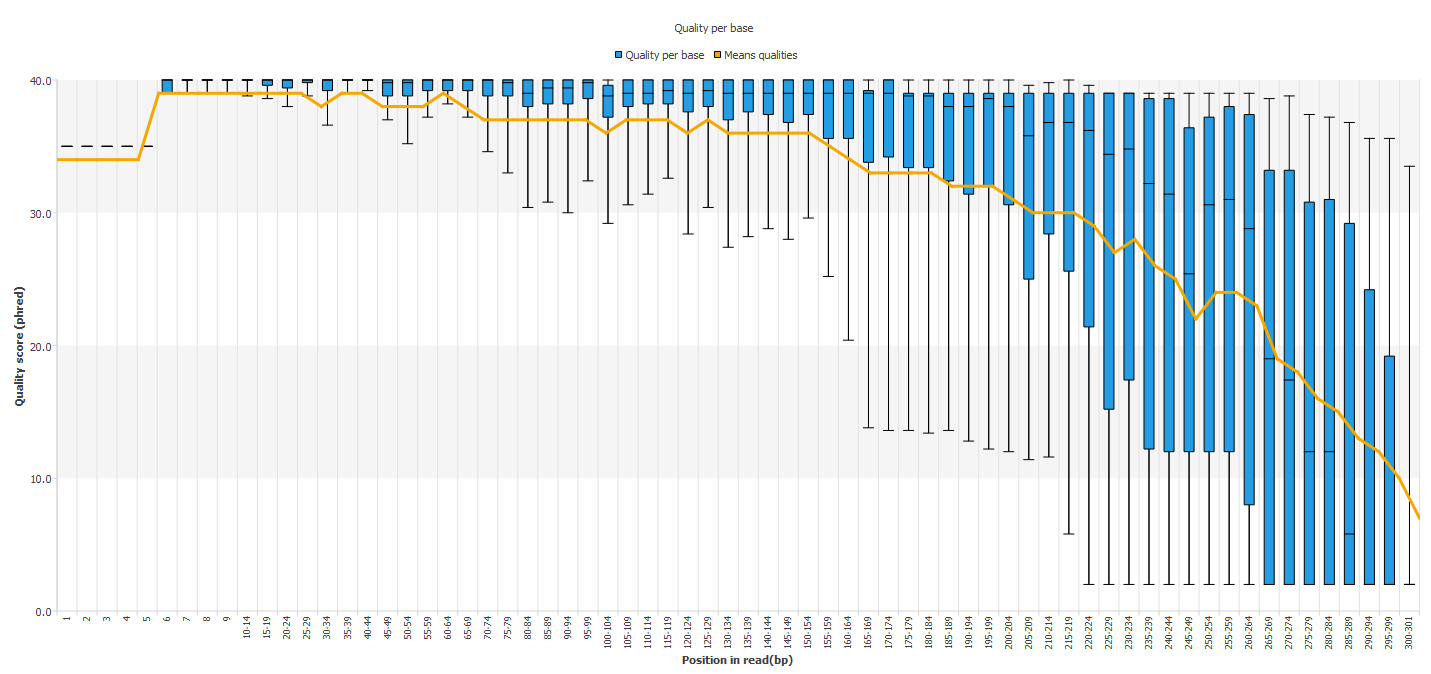
\includegraphics[scale=0.45]{img/1003_forward.png}\hfill
\end{center}
\caption{Qualité par nucléotide des reads forward de l'échantillon 1003. \textbf{Axe X}: la position sur le read. \textbf{Axe Y}: La distribution des qualités}
\label{fastqt}
\end{figure}


\begin{figure}[ht]
\begin{center}
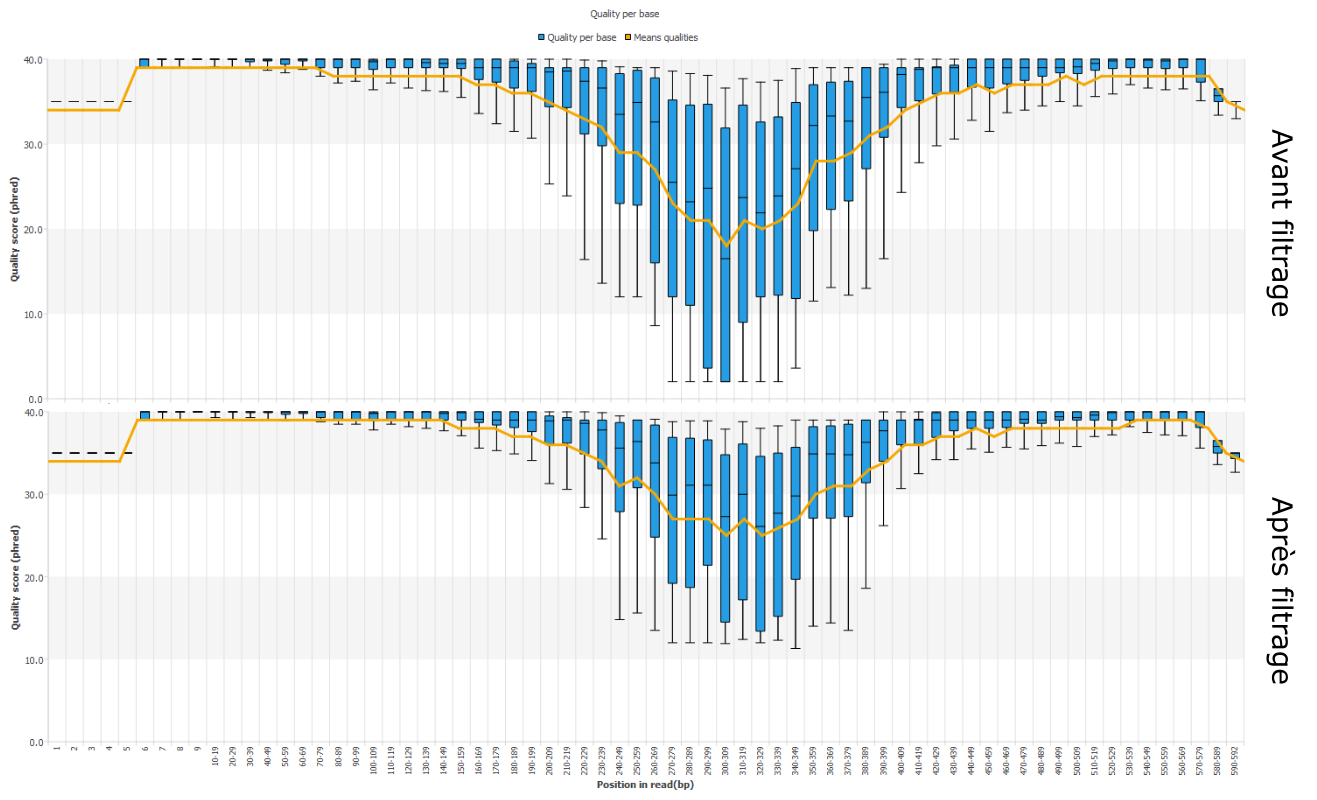
\includegraphics[scale=0.45]{img/duo_merging.png}\hfill
\end{center}
\caption{Qualité par nucléotide des reads fusionné pour l'échantillon 1003}
\label{fastqt_after}
\end{figure}


\subsubsection{Assignement taxonomique}
Après traitement des reads, seulement 49,24 \% (Figure \ref{readgenus}) des reads sont analysable avec des bornes allant de 37,30\% à 61,13\%. La majorité des reads ayant été supprimé lors de l'étape de filtrage.
Au total, 99.88\% des reads analysables ont reçu une assignation taxonomique. La figure \ref{readgenus} montre le nombre de reads assignés par genre bactérien. \\
Au total le pipeline mucobiome s’est exécuté en 1 h 29 sur 40 cœurs et 20 gigaoctets de mémoire contre 21h de calcul sans l’optimisation par déréplication.


\begin{figure}[ht]
\begin{center}
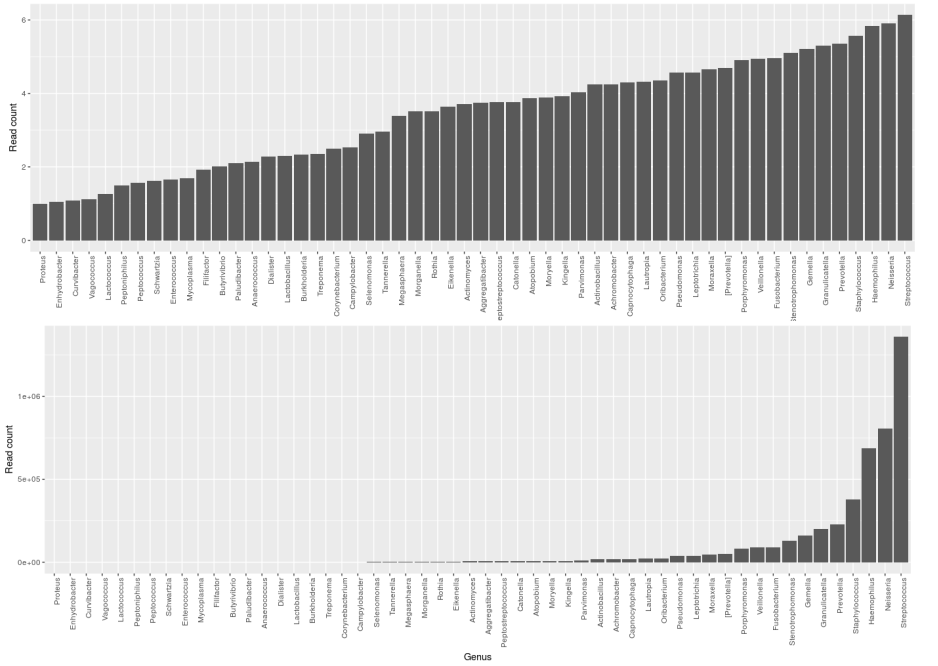
\includegraphics[scale=0.5]{img/read_count_genus_all.png}\hfill
\end{center}
\caption{Nombre de reads par genre bactérien}
\label{readgenus}
\end{figure}


\subsubsection{Qualité d'échantillonnage}
La figure \ref{rarefaction} montre les courbes de raréfaction pour les 188 échantillons.
Dans l'ensemble elles s’aplatissent précocement, témoignant d’un très bon niveau échantillonnage.

\begin{figure}[ht]
\begin{center}
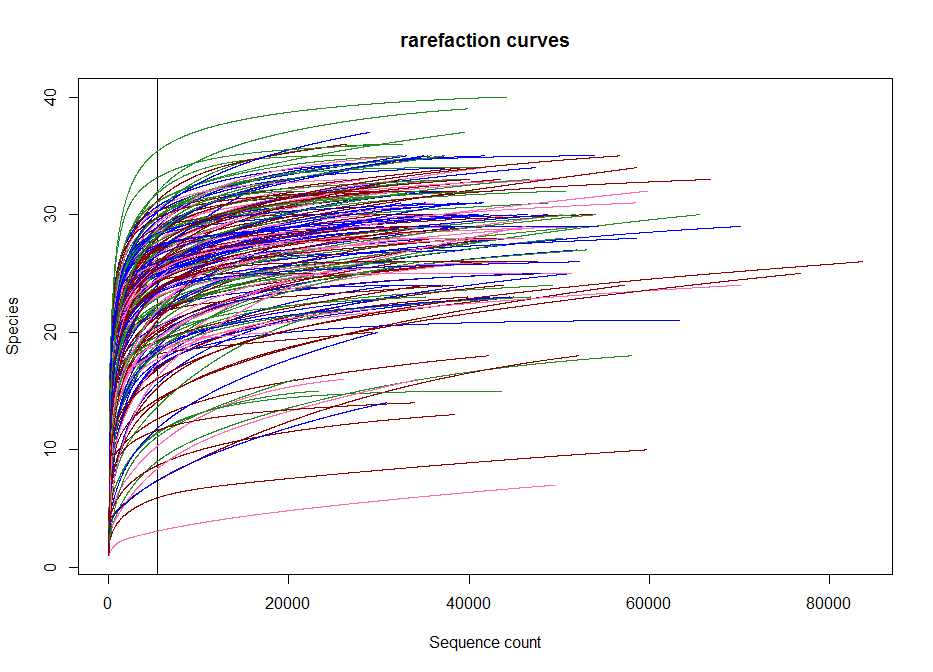
\includegraphics[scale=0.5]{img/rarefaction.png}\hfill
\end{center}
\caption{Courbe de rarefaction}
\label{rarefaction}
\end{figure}


\begin{figure}[!ht]
\begin{center}
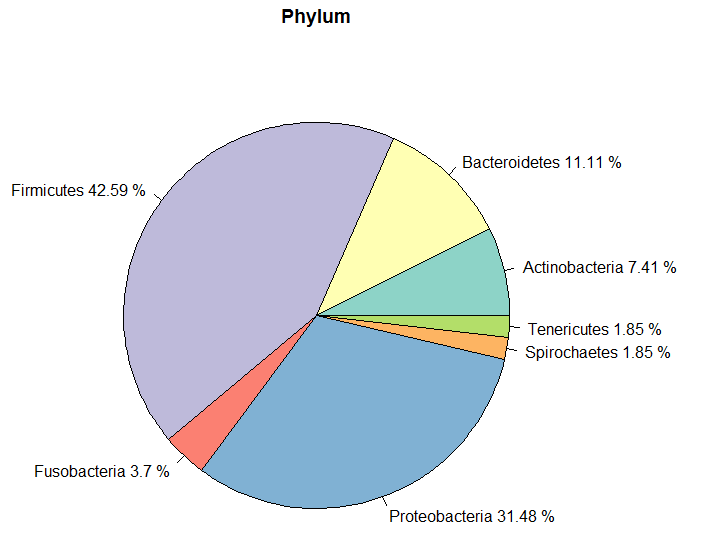
\includegraphics[scale=0.5]{img/phylum.png}\hfill
\end{center}
\caption{Phylum}
\label{phylum}
\end{figure}

\subsection{Diversité globale}
54 genres ( Figure \ref{readgenus} ) et 7 phylums ( Figure \ref{phylum} ) bactériens sont retrouvés dans l'ensemble des échantillons analysés. 
Les trois phylums majoritaires sont \textit{Firmicute} ( 42.59\%) et \textit{Proteobacteria} ( 31.48\%). Parmi les \textit{Firmicutes} majoritaires, on retrouve \textit{Streptococcus} et \textit{Staphylococcus}. Chez les \textit{Protéobacteria} \textit{Neisseria} et \textit{Haemophilus} sont les plus abondantes.
Le tableau de la figure \ref{alltable} résume l'ensemble des résultats en y associant la prévalence des genres bactériens dans les 188 échantillons.
Par exemple \textit{Streptococcus}, \textit{Neisseria}, \textit{Prevotella}, \textit{Granulicatella}, \textit{Gemella}, \textit{Veillonella} et \textit{Fusobacterium} sont très prévalent, car présents dans plus de 185 échantillons.
D’autres sont dominantes, c’est-à-dire qu’ils représentent plus de 90\% du microbiote pulmonaire. Il s’agit de \textit{Streptococcus}, \textit{Neisseria}, \textit{Haemophilus} et \textit{Staphyloccoccus} dans la majorité des cas. \textit{Sténotrophomonas} et \textit{Achromobacter} sont retrouvées dominantes, mais seulement dans 64 et 8 échantillons respectivement. Pseudomonas est retrouvé dans 53 échantillons, dont un, au moins avec une abondance de 25.94\%. \\
Le core microbiota est défini comme l'ensemble des taxons retrouvé dans plus de 50\% des échantillons avec une abondance supérieur à 0,1\%. Il est constitué de 15 genres bactériens ( Figure \ref{core} ). Leurs distribution est illustré dans la figure \ref{violon}.
\textit{Streptococcus} respecte grossièrement une distribution normale qui varie de la quasi-absence à la dominance avec une moyenne de 30\% par échantillon. Neisseria est le deuxième genre le plus abondant avec une moyenne de 18\%.
Les abondances de \textit{Staphylococcus} et \textit{Haemophilus} sont faibles dans la plupart des échantillons. Mais pour quelque un, sont dominant. Les autres genre ont une abondance faible qui varie faiblement. Elles ne sont jamais retrouvé dominante.


\begin{figure}
\begin{center}
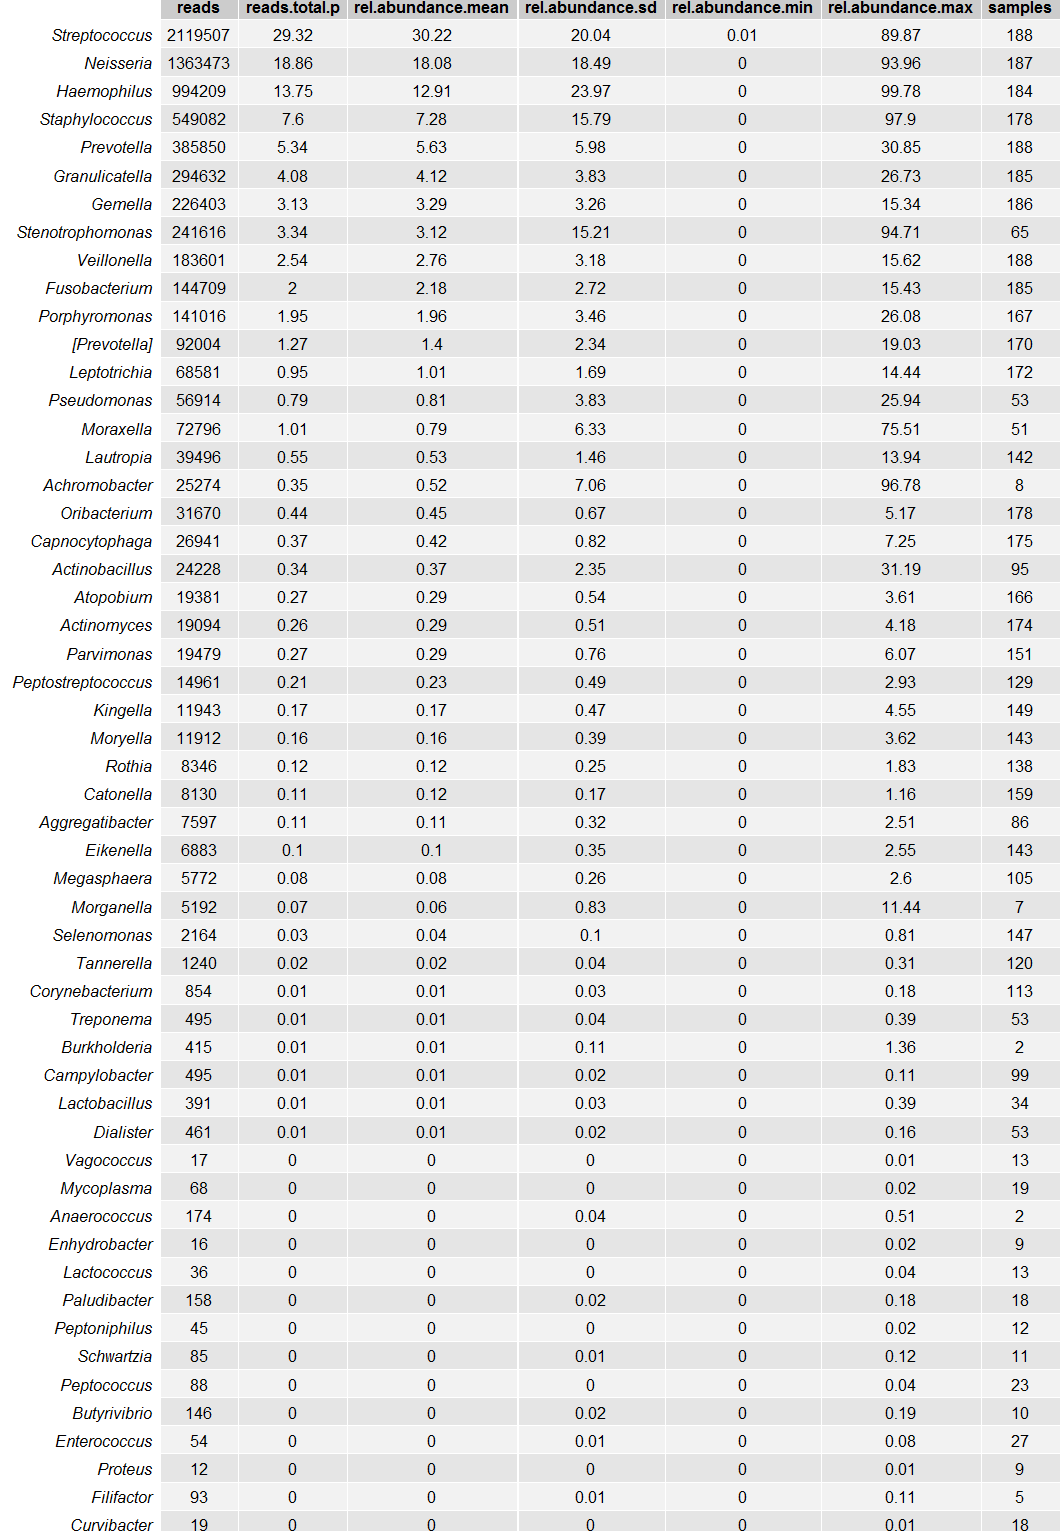
\includegraphics[scale=0.5]{img/all_table.png}\hfill
\end{center}
\caption{Nombre de reads et prévalence des genres bactériens parmis les 188 échantillons}
\label{alltable}
\end{figure}


\begin{figure}[t]
\begin{center}
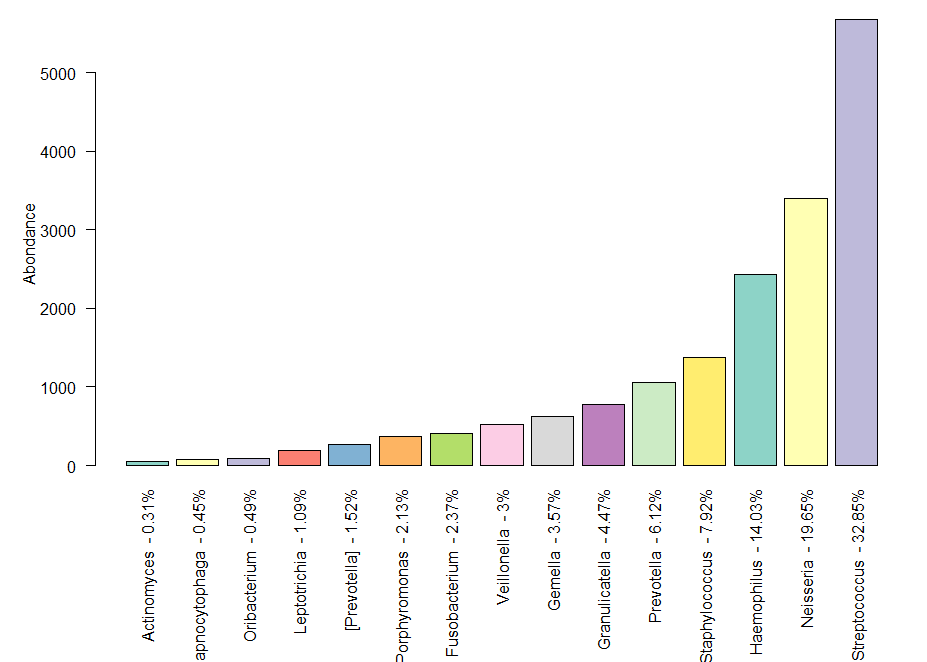
\includegraphics[scale=0.5]{img/core.png}\hfill
\end{center}
\caption{Distribution du Core microbiota dans l'ensemble des échantillons}
\label{core}
\end{figure}



\begin{figure}[t]
\begin{center}
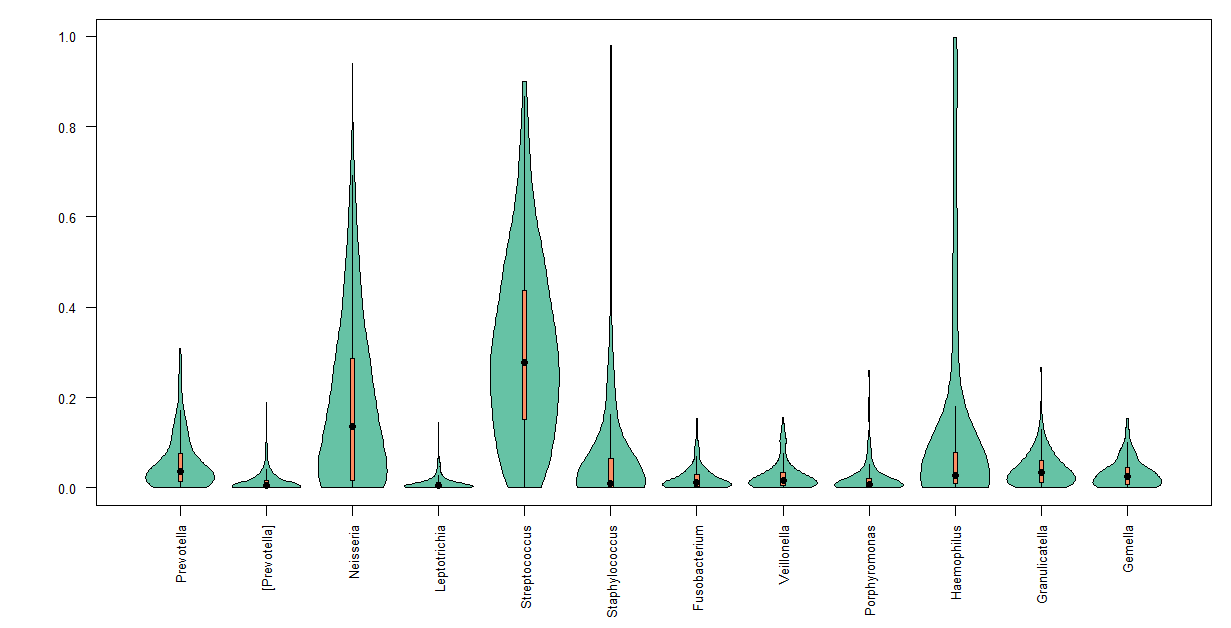
\includegraphics[scale=0.5]{img/variability.png}\hfill
\end{center}
\caption{Distribution du core microbiota}
\label{violon}
\end{figure}





\subsection{Évolution de l'alpha diversité}
Les figures \ref{alphaObs},\ref{alphaChao1} et \ref{alphaShannon} montrent l’évolution des diversités alpha par patient au cours du temps en utilisant 3 indices différents. Les indices Chao1 et Observed reflètent la richesse (nombre de genre) présente dans l’échantillon. Tandis que l’indice de shannon reflète aussi bien la richesse que l’équitabilité des distributions microbiennes.
Les deux premiers graphiques montrent que les échantillons ont un nombre d’espèces pouvant varier de 10 à 40 genres bactériens. La richesse du patient 256 est faible. Celle du patient 26 élevé.
Certains patients ont des richesses stables au court du temps. Le patient 25,26,74 conserve leurs richesses sur plus 5 prélèvements successifs. Le patient 20 et 69 présente une stabilité entrecoupée par des pics de diminution. La richesse du patient 8 diminue progressivement. Le patient 23, 232 et 248 ont des fluctuations chaotiques.
Le graphique de shannon montre que pour un nombre d’espèces constant, leurs distributions varient dans le temps. Par exemple sur le graphique \ref{alphaObs}, le patient 223 contient un nombre de genres relativement stable. En revanche sur le graphique \ref{alphaShannon}, la variabilité de l’indice de shannon du patient 223 indique une distribution des espèces différente entre les échantillons. Seul le patient 26 conserve à la fois une richesse et une distribution stable au court du temps.

\subsection{Evolution des abondances}
Les figures \ref{plotabundancegenre}, \ref{plotabundancephylum} et \ref{plotabundancecurve} nous montre l’évolution des abondances au cours du temps pour chaque patient. Ces graphiques nous permettent d’interpréter plus finement les graphiques d’alpha diversité précédente.
Par exemple la faible richesse du patient 8 est liée à une dominance de \textit{Stenotrophomonas} sur les 4 échantillons.
La perte de diversité du 3ème prélèvement du patient 223 est causée par un \textit{Neisseria} qui devient dominant à plus 80\%.
Le patient 3 montre une diminution progressive \textit{d’Haemophilus} parallèlement à une augmentation de \textit{Streptococcus}.
D’autres échantillons montrent une résilience. Le patient 223 par exemple récupère un microbiote identique après une colonisation complète à \textit{Haemophilus}. \\
Dans l’ensemble, il existe une population de bactéries constante et minoritaire (\textit{Fusobacterium}, \textit{Granulicatella}, \textit{Gemella}, \textit{Veiillonella}, \textit{Parvimonas},\textit{Leptotrichia},\textit{Oribacterium}, \textit{Capnoctophaga},\textit{Catonella}). Et une autre population très fluctuante dans le temps jouant alternativement le rôle de dominant. (\textit{Haemophilus}, \textit{Streptococcus}, \textit{Neissera} et \textit{Prevotella}).
La figure \ref{evolution43} illustre ces propos en montrant l'evolution des abondances du patient 43.
La figure du patient \ref{evolution54} est mis également à titre exemple, car elle montre l’apparition de \textit{Pseudomonas Aeruginosa}. \\
L’ensemble des graphiques est disponible sur cette adresse.

\subsection{Corrélation entre genre }
La figure \ref{correlation} montre les corrélations linéaires réalisées entre les genres du core microbiota. La corrélation la plus forte est entre Prevotella et Veillonella avec un coefficient de Pearson à 0.60 (p<0.5).  Streptococcus et Haemophilus evolue dans le sens inverse avec un coefficient à -0.41  (p<0.5). 
 

\begin{figure}
\begin{center}
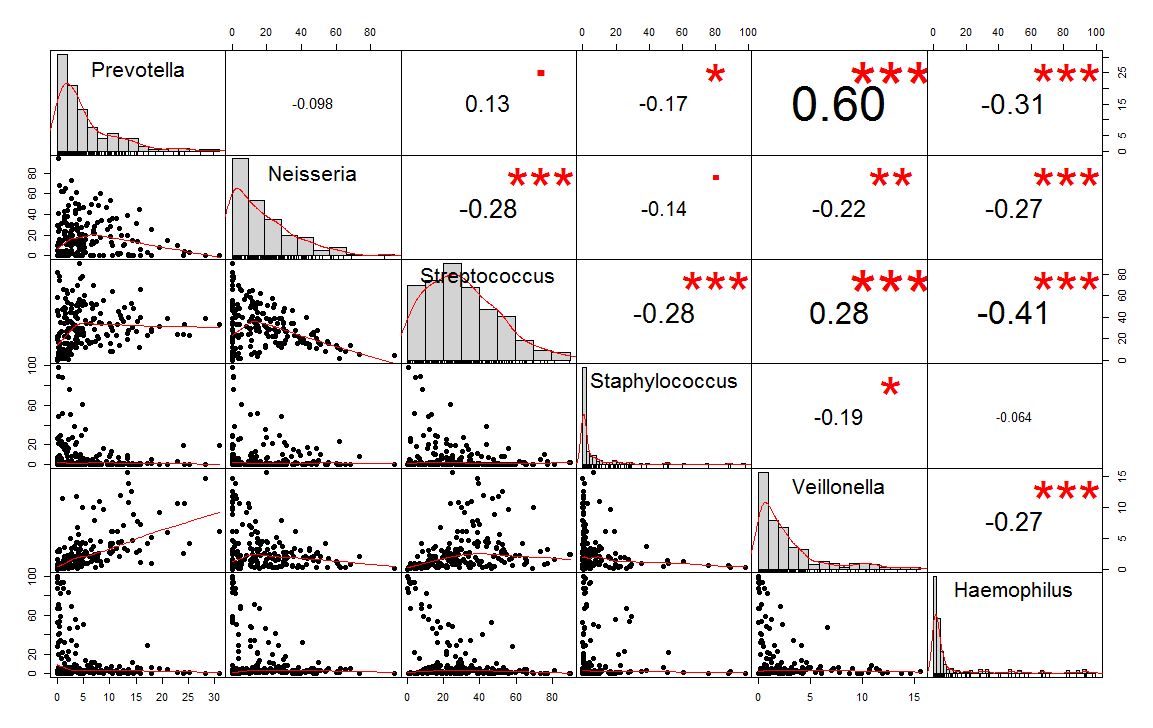
\includegraphics[scale=0.50]{img/small_correlation.png}\hfill
\end{center}
\caption{Corrélation des abondances entre les genres du core microbiota}
\label{correlation}
\end{figure}




\begin{figure}
\begin{center}
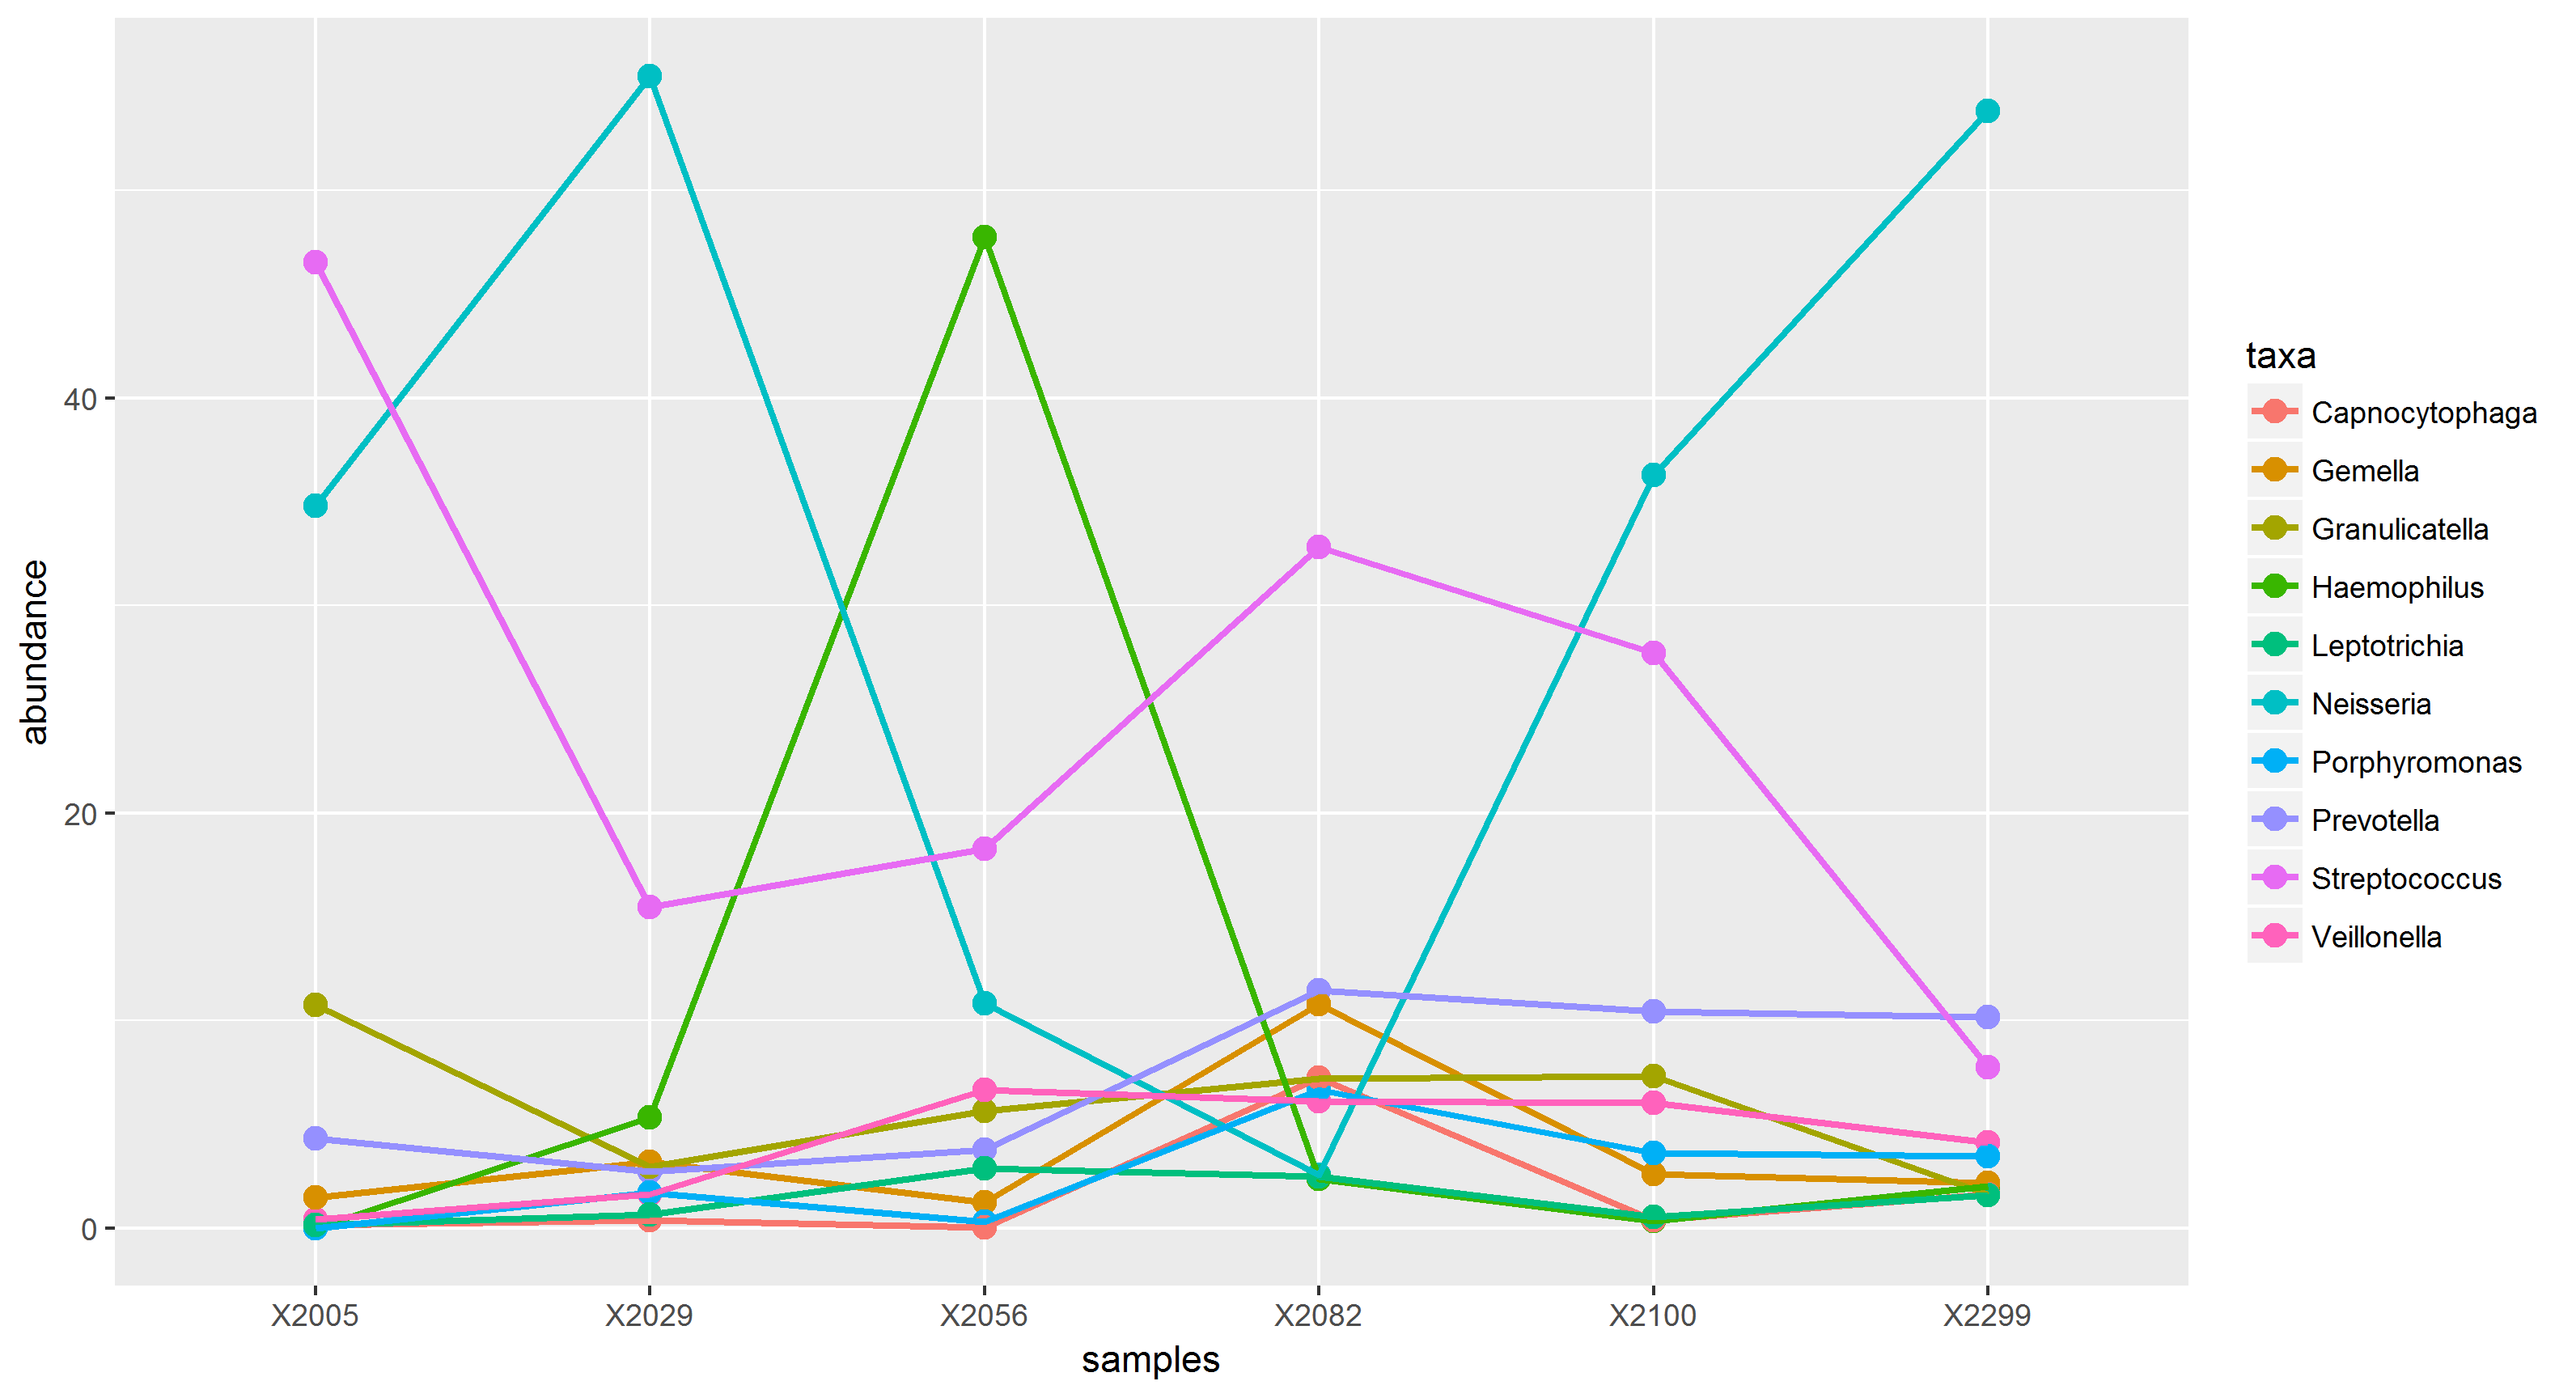
\includegraphics[scale=0.60]{img/curve_043.png}\hfill
\end{center}
\caption{Evolution des abondances pour le patient 43. Notez la population stable et la population fluctuante}
\label{evolution43}
\end{figure}

\begin{figure}
\begin{center}
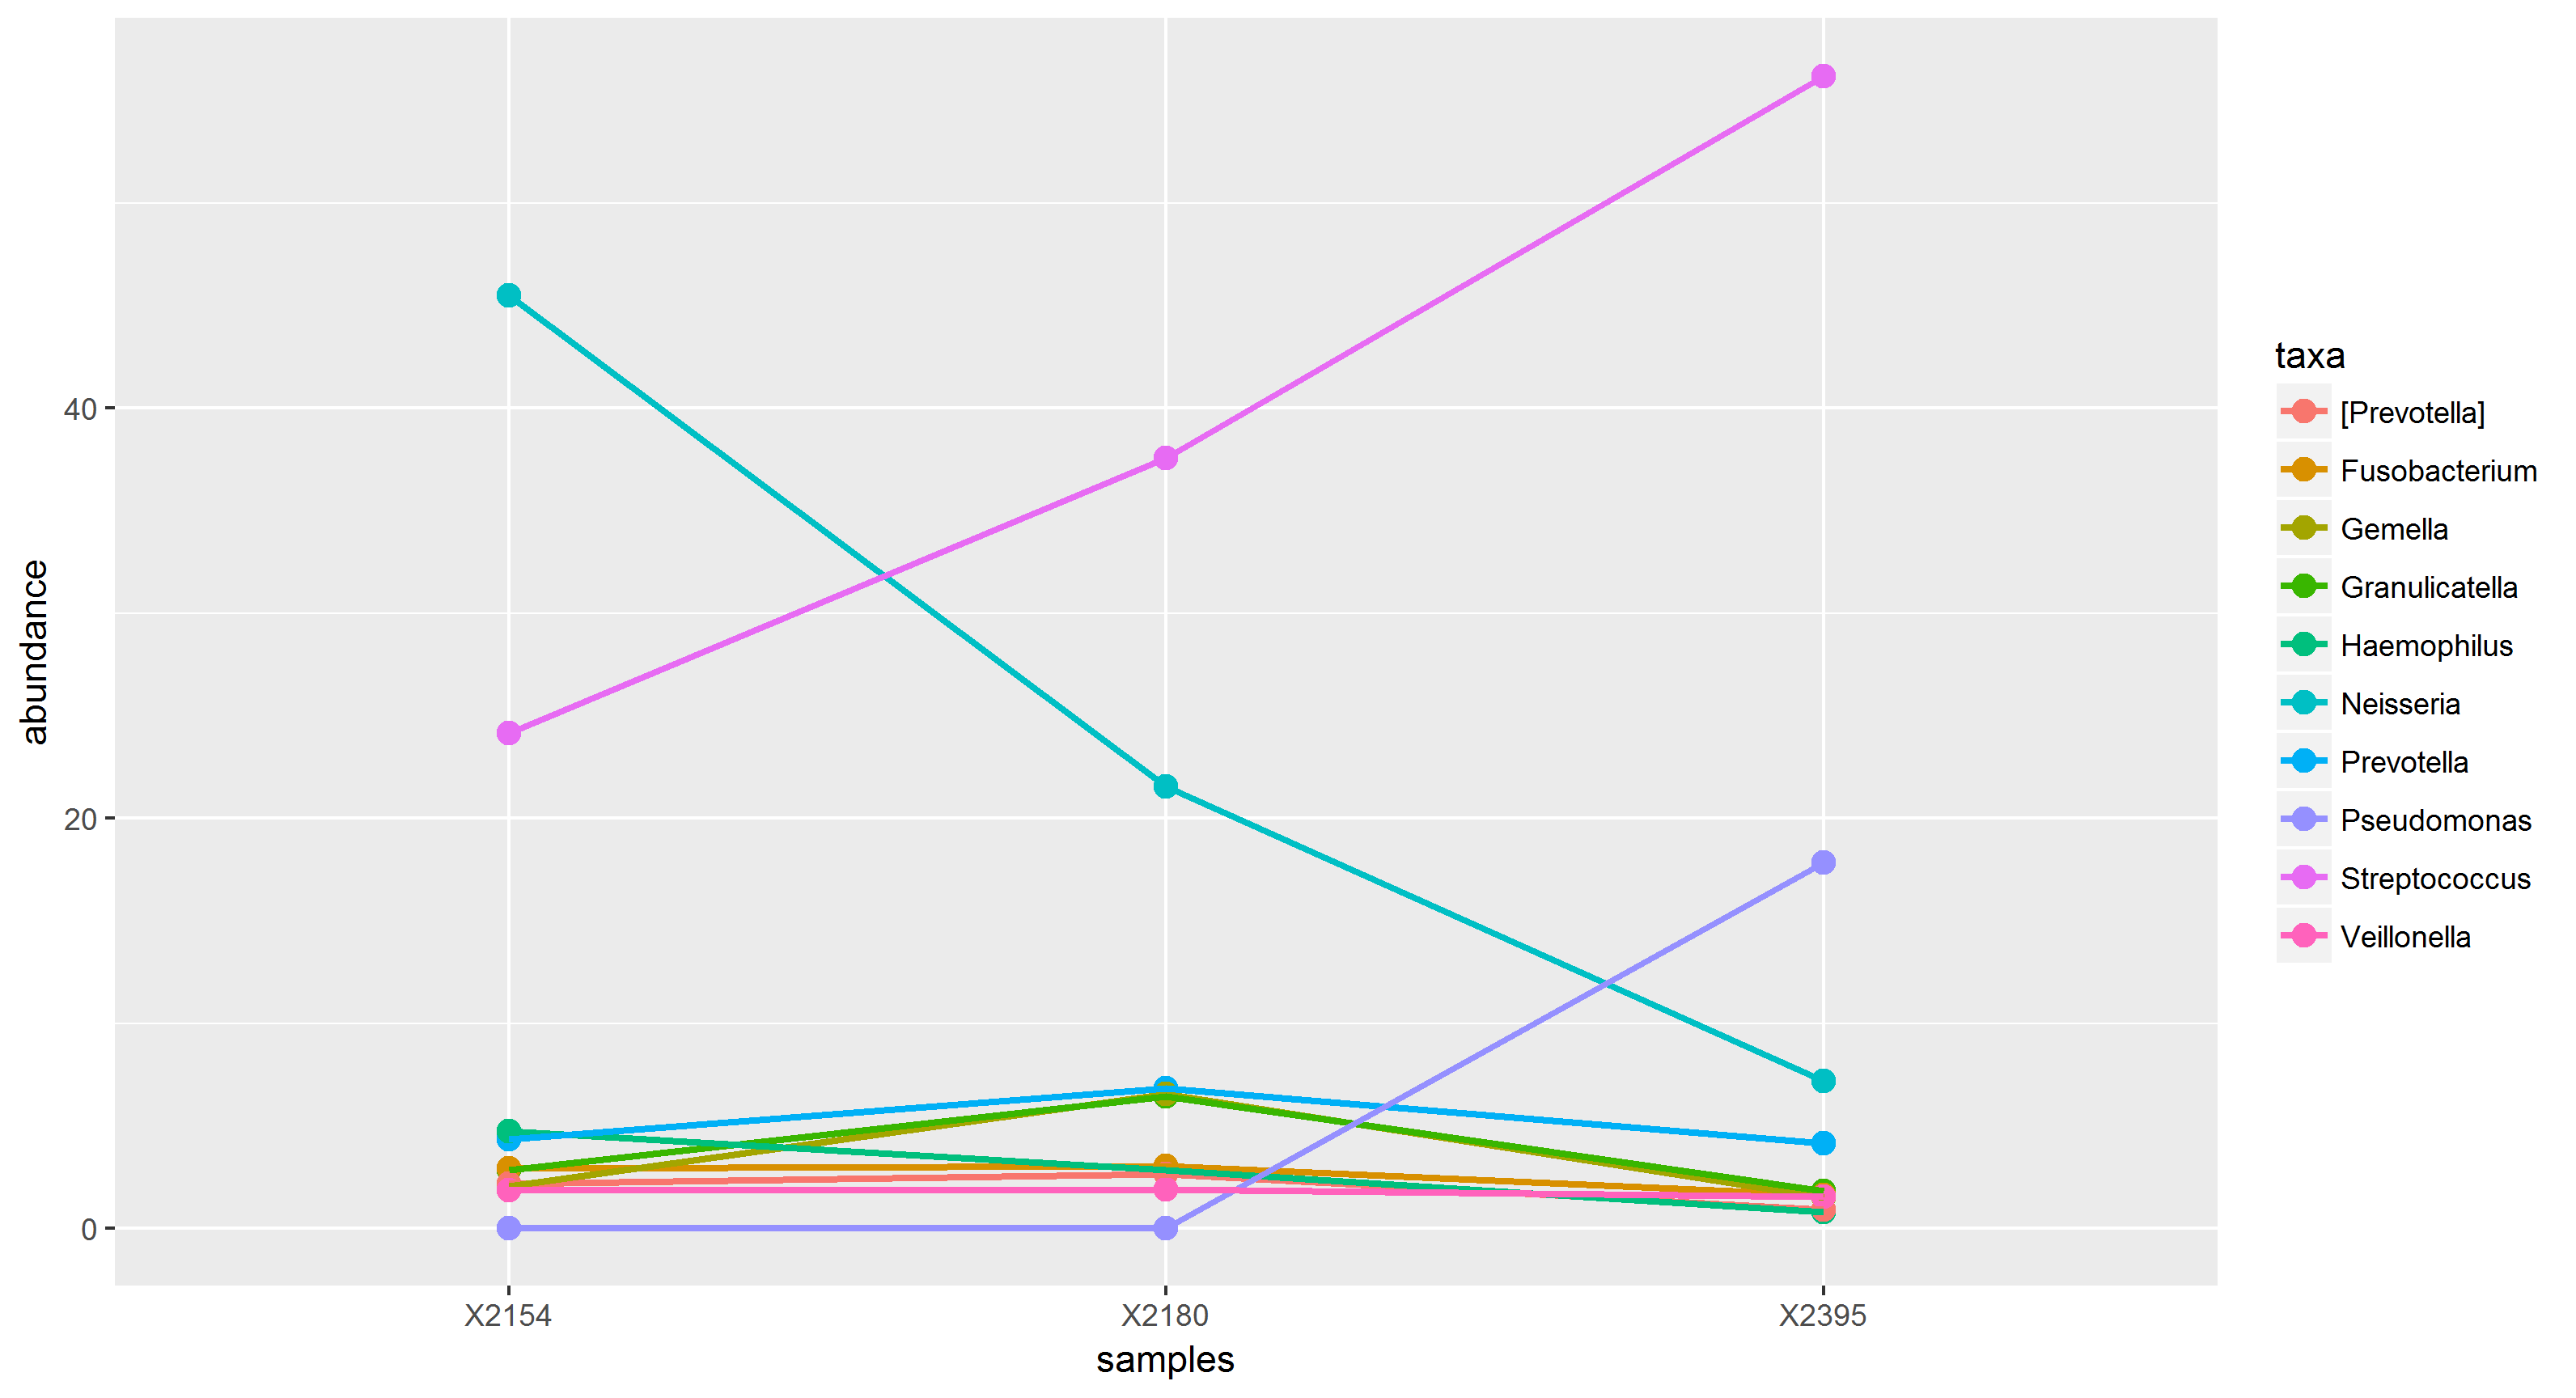
\includegraphics[scale=0.60]{img/curve_054.png}\hfill
\end{center}
\caption{Evolution des abondances pour le patient 54. Notez l'apparition de \textit{Pseudomonas} dans le dernier échantillon}
\label{evolution54}
\end{figure}



\subsection{Beta Diversité}
La bêta diversité sur l’ensemble des échantillons a été réalisé par une méthode d’ordination de type PCA en utilisant les distances de Bray-curtis ( Figure \ref{ordination} et \ref{ordination2} ).
2 axes principaux expliquent respectivement 28.5\% et 17.4\% de la variabilité.
Certains échantillons d’un même patient sont très proches sur le graphique d’ordination. Par exemple le patient 69 et 003 ont des échantillons dont les points se confondent.
Aucun des paramètres comme âge, le sexe, le poids, la prise d'antibiotique et le type de mutation n’a mis en évidence des groupes distincts de microbiote. La variabilité est expliqué principalement par la dominance des genres Neisseria, Streptococcus et Haemophilus.
La diversité des microbiotes des échantillons Free ont une diversité plus faible que les échantillons Never. 


\begin{figure}
\begin{center}
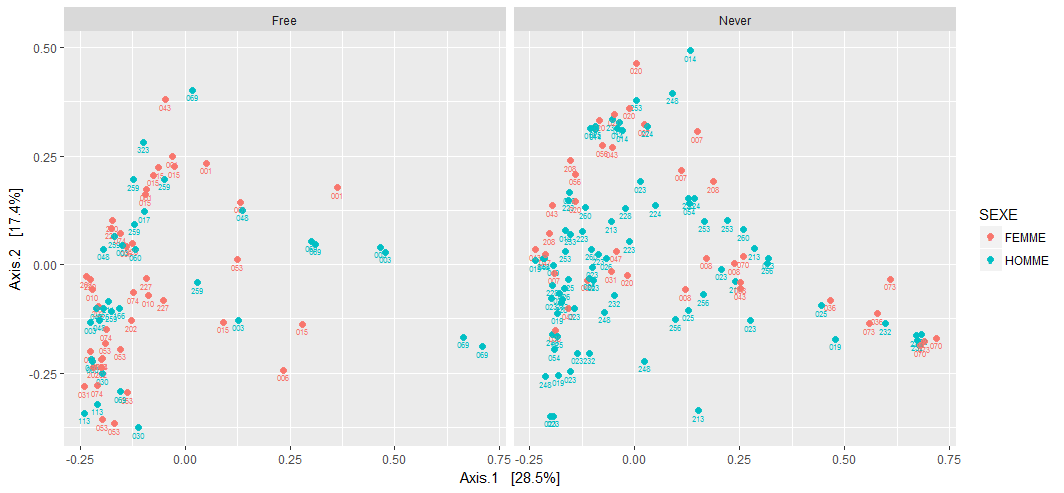
\includegraphics[scale=0.60]{img/oordination_new.png}\hfill
\end{center}
\caption{Analyse multivarié ( PCA + Bray curtis) sur les 188 échantillons. Chaque point est un échantillon labelisé par l'identifiant du patient. A gauche les échantillons Free. A droite les échantillons Never. }
\label{ordination}
\end{figure}

\begin{figure}
\begin{center}
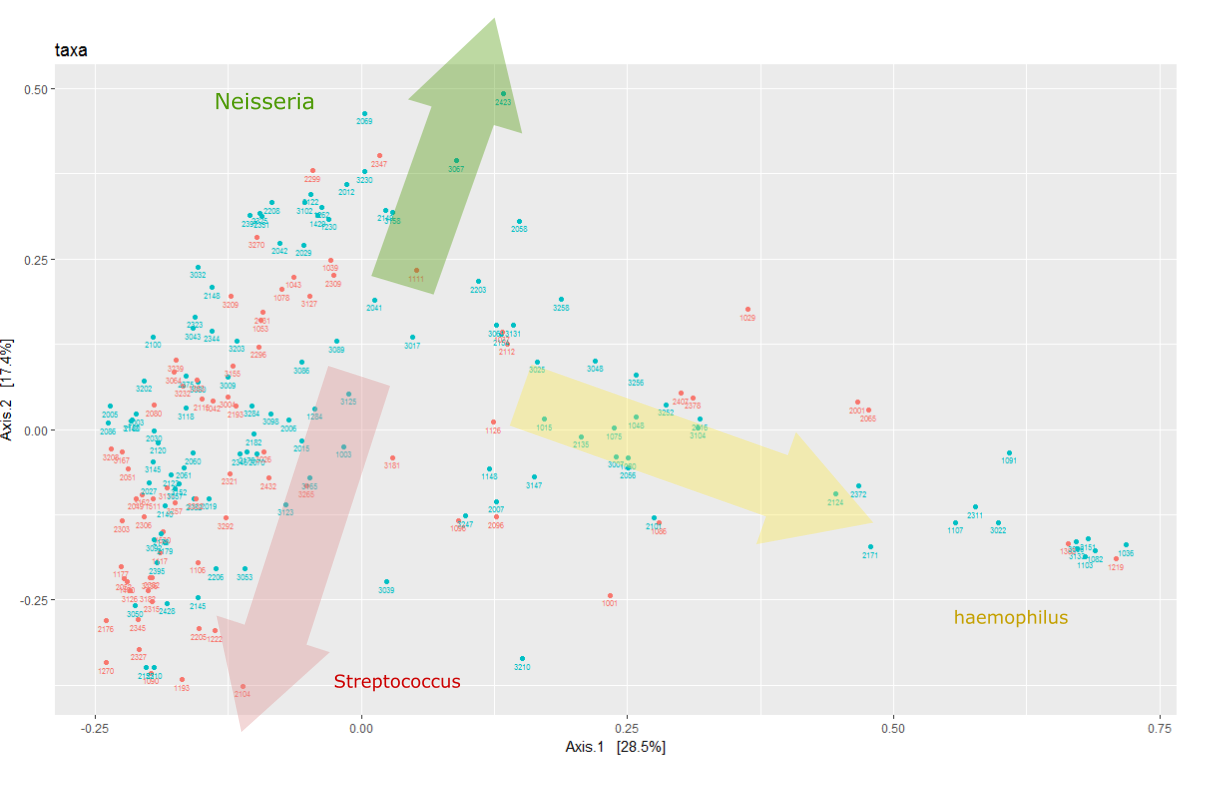
\includegraphics[scale=0.40]{img/Capture.png}\hfill
\end{center}
\caption{Analyse multivarié ( PCA + Bray curtis) sur les 188 échantillons. Chaque point est un échantillon labelisé par l'identifiant du patient.}
\label{ordination2}
\end{figure}


Discussion
LA RÉSOLUTION TEMPORALE n’EST PAS ASSEZ GRANDE
Population d’attaque et population locale
Notion des 2 calques papiers
On retrouve du corynébactérium …
Conclusion




\begin{figure}
\begin{center}
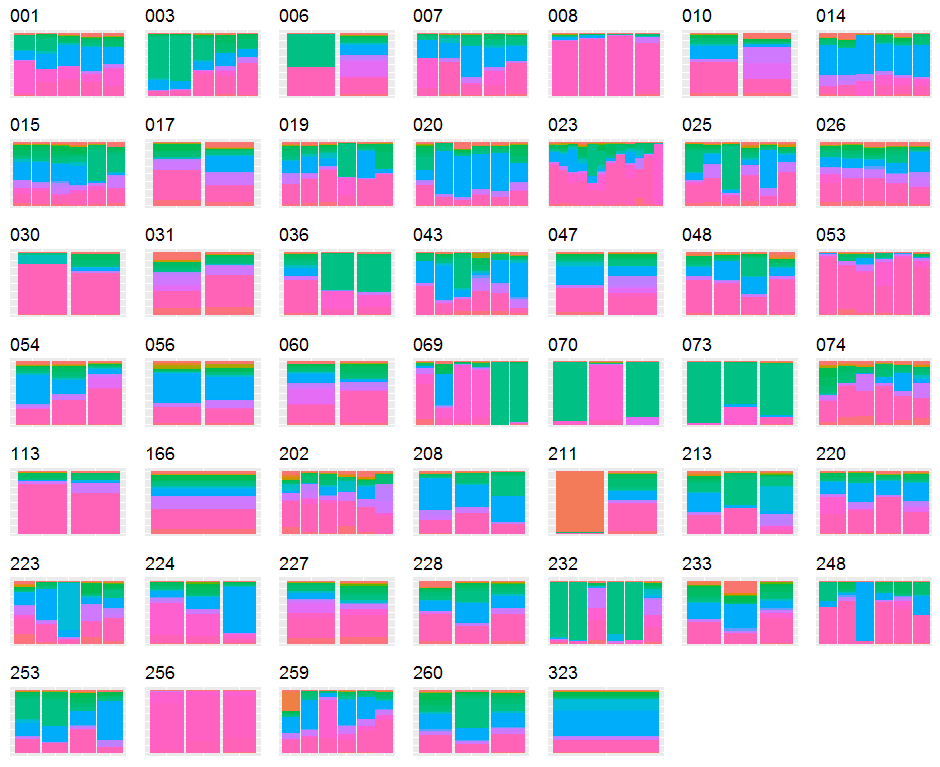
\includegraphics[scale=0.60]{img/enfin_barplot_genus_norm.png}\hfill
\end{center}
\caption{Evolution des abondances par genre}
\label{plotabundancegenre}
\end{figure}

\begin{figure}
\begin{center}
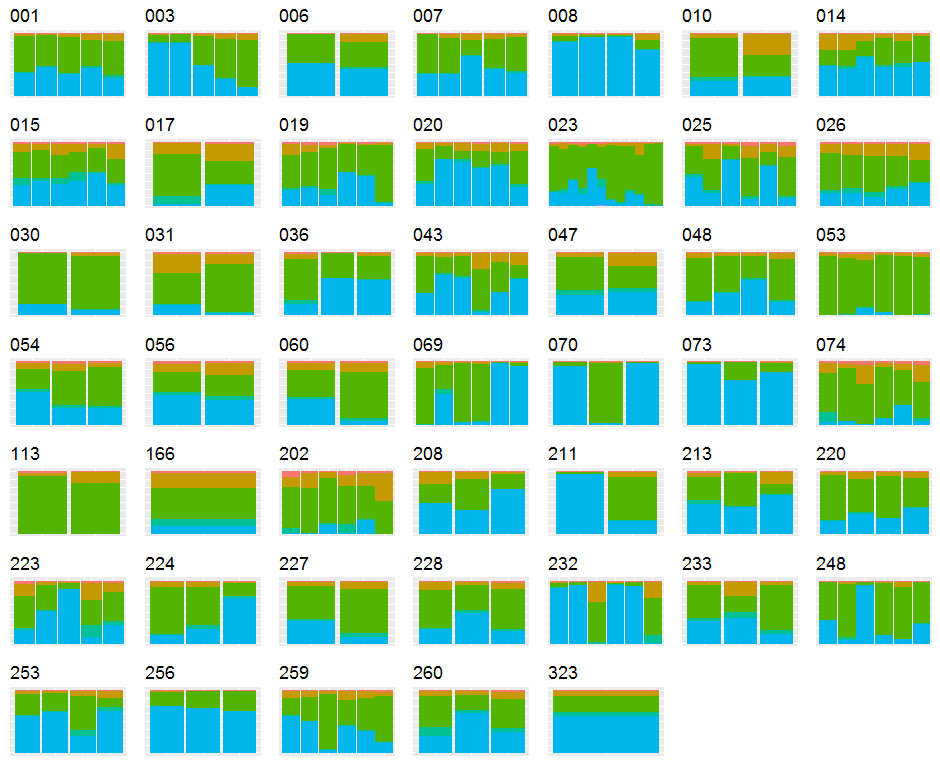
\includegraphics[scale=0.60]{img/enfin_barplot_phylum_norm.png}\hfill
\end{center}
\caption{Evolution des abondances par phylum}
\label{plotabundancephylum}
\end{figure}


\begin{figure}
\begin{center}
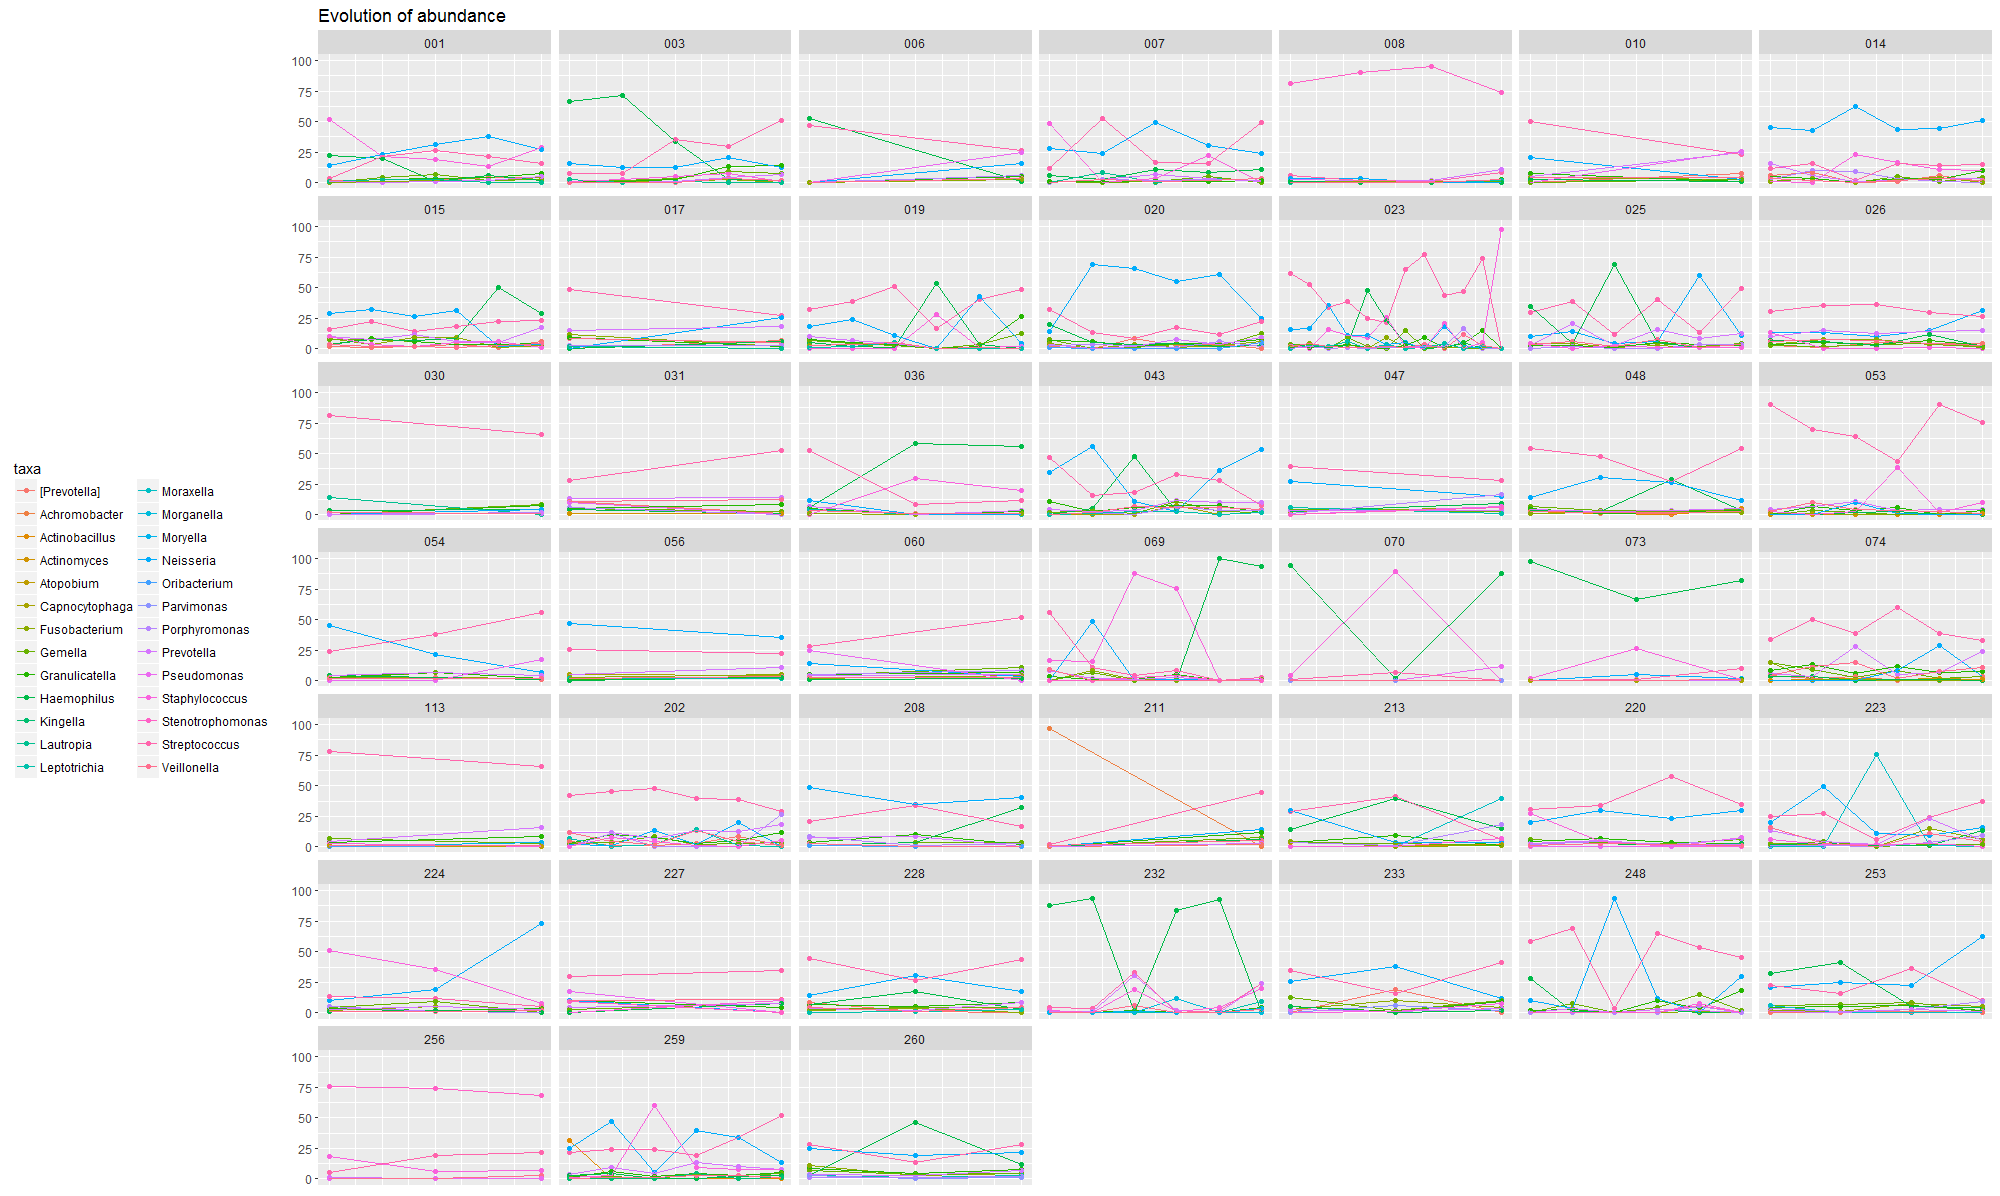
\includegraphics[scale=0.40,angle=90]{img/evolution_abundance.png}\hfill
\end{center}
\caption{Evolution des abondances par genre}
\label{plotabundancecurve}
\end{figure}


\begin{figure}
\begin{center}
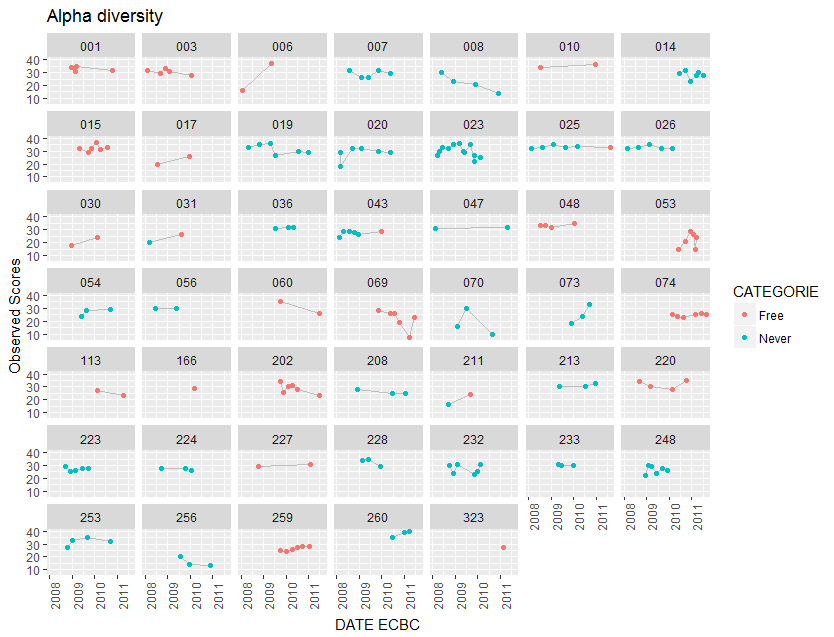
\includegraphics[scale=0.80]{img/alpha_observed.png}\hfill
\end{center}
\caption{Evolution du nombre d'espèces par patient en fonction du temps}
\label{alphaObs}
\end{figure}


\begin{figure}
\begin{center}
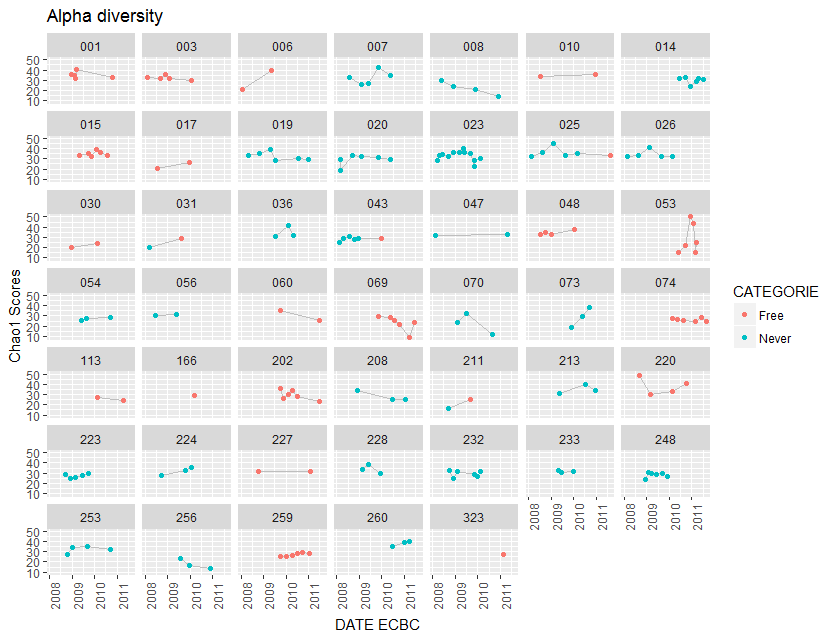
\includegraphics[scale=0.80]{img/alpha_chao1.png}\hfill
\end{center}
\caption{Evolution de l'indice de Chao1 par patient en fonction du temps}
\label{alphaChao1}
\end{figure}

\begin{figure}
\begin{center}
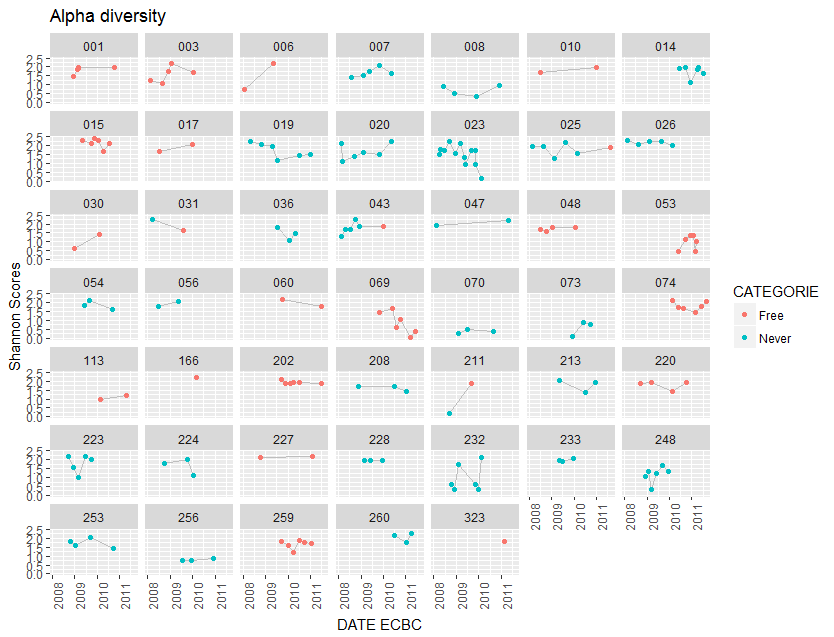
\includegraphics[scale=0.80]{img/alpha_shannon.png}\hfill
\end{center}
\caption{Evolution de l'indice de Shanon par patient en fonction du temps}
\label{alphaShannon}
\end{figure}







\section{Discussion}


\section{Conclusion}




\newpage


\bibliographystyle{plain}
\bibliography{biblio}

\end{document}
